%%%%%%%%%%%%%%%%%%%%%%%%%%%%%%%%%%%%%%%%%%%%%%%%%%%%%%%%%%%%%%%%%%%%%%%%
% Copyright (c) 2023 The authors
%
% This work is licensed under a
% Creative Commons Attribution-ShareAlike 4.0 International License.
%
% You should have received a copy of the license along with this
% work. If not, see <http://creativecommons.org/licenses/by-sa/4.0/>.
%%%%%%%%%%%%%%%%%%%%%%%%%%%%%%%%%%%%%%%%%%%%%%%%%%%%%%%%%%%%%%%%%%%%%%%%

\documentclass{article}

%% Packages
\usepackage{arxiv}
\usepackage{authblk}
\usepackage[T1]{fontenc}   
\usepackage{amsthm}
\usepackage{amsmath}
\usepackage[english]{babel}
\usepackage{mathtools}
\usepackage{amssymb}
\usepackage{microtype}
\usepackage[table,usenames,dvipsnames]{xcolor}
\usepackage{booktabs}
\usepackage{multirow}
\usepackage{placeins}
\usepackage{bm}
\usepackage[authoryear]{natbib}
\usepackage[
  colorlinks,
  linkcolor=blue,
  citecolor=blue,
  urlcolor=blue,
  filecolor=blue,
  backref=page
]{hyperref}
\usepackage{graphicx}

%% Graphics path
\graphicspath{%
  {./},
  {./figures}
}

%% Bibliography style
\bibliographystyle{ba.bst}

%% Show links only in year in citations
\citefix{} % defined in arxiv.sty

%% Insert space before backref pages in reference list
\NewCommandCopy{\oldbackref}{\backref}
\renewcommand*{\backref}[1]{
  \hspace{0.1em}\oldbackref{#1}
}

%% Author block typeset
\renewcommand\Authfont{\bfseries}
\setlength{\affilsep}{0em}

%% Space between rows in tables
\renewcommand{\arraystretch}{1.2}

%% Emphasis 
\newcommand\firstcolor[1]{\textbf{#1}}
\newcommand\secondcolor[1]{{\color{RoyalBlue}{#1}}}

%% Bold letters in math mode 
\makeatletter
\g@addto@macro\bfseries{\boldmath}
\makeatother

%% Maths settings
\numberwithin{equation}{section}
\theoremstyle{plain}
\newtheorem{theorem}{Theorem}[section]
\newtheorem{proposition}{Proposition}[section]
\newtheorem{condition}{Condition}[section]
\newtheorem{definition}{Definition}[section]

%% Custom commands
\renewcommand{\epsilon}{\varepsilon}

\newcommand{\N}{\mathbb{N}}
\newcommand{\R}{\mathbb{R}}
\newcommand{\E}{\mathbb{E}}
\newcommand{\Hcal}{\mathcal{H}}
\newcommand{\tTheta}{\tilde{\Theta}}
\newcommand{\I}{\mathbb{I}}

\DeclareMathOperator{\Var} {Var}
\DeclareMathOperator{\Cov} {Cov}
\DeclareMathOperator{\supp} {supp}

\newcommand\dotprod[2]{\left\langle#1,#2\right\rangle}

%% Title and author information
\title{A Bayesian approach to functional regression: theory and computation}

\date{December 21, 2023}

\newbox{\orcid}\sbox{\orcid}{
\includegraphics[scale=0.06]{orcid.pdf}} 
\author[1,2]{%
	\href{https://orcid.org/0000-0003-0728-7748}{\usebox{\orcid}\hspace{1mm}José R.~Berrendero\thanks{\texttt{\href{mailto:joser.berrendero@uam.es}{joser.berrendero@uam.es}}}}%
}
\author[1]{%
	\href{https://orcid.org/0009-0004-7554-9193}{\usebox{\orcid}\hspace{1mm}Antonio Coín\thanks{\texttt{\href{mailto:antonio.coin@uam.es}{antonio.coin@uam.es}} (corresponding author)}}%
}
\author[1,2]{%
	\href{https://orcid.org/0000-0002-7993-0096}{\usebox{\orcid}\hspace{1mm}Antonio Cuevas\thanks{\texttt{\href{mailto:antonio.cuevas@uam.es}{antonio.cuevas@uam.es}}}}%
}
\affil[1]{Departamento de Matemáticas, Universidad Autónoma de Madrid (UAM), Madrid, Spain}
\affil[2]{Instituto de Ciencias Matemáticas ICMAT (CSIC-UAM-UC3M-UCM), Madrid, Spain}
\newcommand\shortauthor{J. R. Berrendero, A. Coín and A. Cuevas}

%% PDF metadata
\hypersetup{
pdftitle={A Bayesian approach to functional regression: theory and computation},
pdfsubject={Preprint},
pdfauthor={José R.~Berrendero, Antonio Coín, Antonio Cuevas},
pdfkeywords={functional data, linear regression, logistic regression, reproducing kernel Hilbert space, Bayesian inference, posterior consistency},
}

%%%%%%%%%%%%%%%%%%%%%%%%%%%%%%%%%%%%%%%%%%%%%%%%%%%%%%%%%%%%%%%%%%%%%%%%%%
%% Document body
%%%%%%%%%%%%%%%%%%%%%%%%%%%%%%%%%%%%%%%%%%%%%%%%%%%%%%%%%%%%%%%%%%%%%%%%%%

\begin{document}

  \maketitle

  %% Abstract
  \begin{abstract}
    We propose a novel Bayesian methodology for inference in functional linear and logistic regression models based on the theory of reproducing kernel Hilbert spaces (RKHS's). These models build upon the RKHS associated with the covariance function of the underlying stochastic process, and can be viewed as a finite-dimensional approximation to the classical functional regression paradigm. The corresponding functional model is determined by a function living on a dense subspace of the RKHS of interest, which has a tractable parametric form based on linear combinations of the kernel. By imposing a suitable prior distribution on this functional space, we can naturally perform data-driven inference via standard Bayes methodology, estimating the posterior distribution through Markov chain Monte Carlo (MCMC) methods. In this context, our contribution is two-fold. First, we derive a theoretical result that guarantees posterior consistency in these models, based on an application of a classic theorem of Doob to our RKHS setting. Second, we show that several prediction strategies stemming from our Bayesian formulation are competitive against other usual alternatives in both simulations and real data sets, including a Bayesian-motivated variable selection procedure.
  \end{abstract}

  %% Keywords
  \keywords{functional data \and linear regression \and logistic regression \and reproducing kernel Hilbert space \and Bayesian inference \and posterior consistency}

%%%%%%%%%%%%%%%%%%%%%%%%%%%%%%%%%%%%%%%%%%%%%%%%%%%%%%%%%%%%%%%%%%


\section{Introduction}\label{sec:intro}

The problem of predicting a scalar response from a functional covariate is one that has gained traction over the last few decades, as more and more data is being generated with an ever-increasing level of granularity in the measurements. While in principle the functional data could simply be regarded as a discretized vector in a very high dimension, there are often many advantages in taking into account the functional nature of the data, ranging from modeling the possibly high correlation among points that are close in the domain, to extracting information that may be hidden in the derivatives of the function in question. As a consequence, numerous proposals have arisen on how to suitably deal with functional data, all of them encompassed under the term Functional Data Analysis (FDA), which essentially explores statistical techniques to process, model and make inference on data varying over a continuum. A partial survey on such methods is \citet{cuevas2014partial} or \citet{goia2016introduction}, while a more detailed exposition of the theory and applications can be found for example in \citet{ramsay2005functional} or \citet{hsing2015theoretical}.

FDA is undoubtedly an active area of research, which finds applications in a wide variety of fields, such as biomedicine, finance, meteorology or chemistry \citep[see for example][]{ullah2013applications}. Accordingly, there are many recent contributions on how to tackle functional data problems, both from a theoretical and practical standpoint. Chief among them is the approach of reducing the problem to a finite-dimensional one, for example using a truncated basis expansion or spline interpolation methods \citep[e.g.][]{muller2005generalized, aguilera2013comparative}. At the same time, much effort has also been put into the task of building a sound theoretical basis for FDA, generalizing different concepts to the infinite-dimensional framework. Examples of this endeavor include the definition of centrality measures and depth-based notions for functional data \citep[e.g.][]{fraiman2001trimmed, cuevas2007robust, lopez2009concept}, an ANOVA test for functional data \citep{cuevas2004anova}, a purely functional partial least squares algorithm \citep{delaigle2012methodology}, a functional Mahalanobis distance \citep[e.g.][]{galeano2015mahalanobis, berrendero2020mahalanobis}, or an extension of Fisher's discriminant analysis for random functions \citep[e.g.][]{james2001functional, shin2008extension}, among many others. Moreover, additional non-parametric methods for functional prediction and classification were notably explored in \citet{ferraty2006nonparametric}. As the name suggests, FDA techniques are heavily inspired by functional analysis tools and methods: Hilbert spaces, orthonormal systems, linear operators, and so on. Incidentally, a notion that also intersects with the classical theory of machine learning and pattern recognition, and that has gained popularity in recent years, is that of reproducing kernel Hilbert spaces (RKHS's) and their applications in functional data problems (see for example \citealp{yuan2010reproducing} or \citealp{berrendero2018use, berrendero2020general}).

On the other hand, Bayesian inference methods are ubiquitous in the realm of statistics, and their usual non-parametric approach also makes use of random functions, though in a slightly different manner than in the FDA context. However, while there are recent works in the literature that offer a Bayesian treatment of functional data \citep[e.g.][]{scarpa2009bayesian, crainiceanu2010bayesian, shi2011gaussian, kang2023fast}, there is still no systematic approach to Bayesian methodologies within the FDA framework. It is precisely at this relatively unexplored intersection between FDA and Bayesian methods that our work is aimed. In particular, our goal is to study functional regression problems, which are the infinite-dimensional equivalents of the usual regression problems that appear in statistics and machine learning. We follow the path started by \citet{ferguson1974prior} of setting a prior distribution on a functional space, but in our case we take a particular RKHS as the ambient space, obtaining functional regression models that allow for a simple yet efficient Bayesian treatment of functional data. Moreover, we also study the basic theoretical question of posterior consistency in these RKHS models within the proposed Bayesian framework. The concepts of consistency and posterior concentration are a kind of frequentist validation that have arguably been an active point of research in the last few decades, particularly in infinite-dimensional settings \citep[see][]{amewou2003posterior, ghosh2003bayesian, choi2008remarks}, and also in the functional regression case \citep[e.g.][]{lian2016posterior,abraham2020posterior}. To put it simply, posterior consistency ensures that with enough samples, the Bayesian updating mechanism works as intended and the posterior distribution eventually concentrates around the true value of the parameters, supposing the model is well specified. We leverage the properties of RKHS's and existing techniques, mainly by \citet{nobile1994bayesian} and \citet{miller2023consistency}, to show that posterior consistency holds in our RKHS models under some mild identifiability conditions, thus providing a strong and coherent background to our Bayesian approach. Finally, this theoretical side is complemented by extensive experimentation that demonstrates the predictive performance of the proposed functional regression models, especially when compared with other usual frequentist methods.

\subsubsection*{\(L^2\)-models, shortcomings and alternatives}

In this work we are concerned with functional linear and logistic regression models, that is, situations where the goal is to predict a continuous or dichotomous variable from functional observations. Even though these problems can be formally stated with almost no differences from their finite-dimensional counterparts, there are some fundamental challenges as well as some subtle drawbacks that emerge as a result of working in infinite dimensions. To set a common framework, we will consider throughout a scalar response variable \(Y\) (either continuous or binary) which has some dependence on a stochastic \(L^2\)-process \(X=X(t)=X(t, \omega)\) with trajectories in \(L^2[0, 1]\). We will further suppose that \(X\) is centered, that is, its mean function \(m(t)=\E[X(t)]\) vanishes for all \(t\in[0,1]\). In addition, when prediction is our ultimate objective, we will tacitly assume the existence of a \textit{labeled} data set \(\mathcal D_n =\{(X_i, Y_i): i=1,\dots, n\}\) of independent observations from \((X, Y)\), and our aim will be to accurately predict the response corresponding to unlabeled samples from \(X\).

The most common scalar-on-function linear regression model is the classical \(L^2\)-model, widely popularized since the first edition (1997) of the monograph by~\citet{ramsay2005functional}. It can be seen as a generalization of the usual finite-dimensional model, replacing the scalar product in \(\R^d\) for that of the functional space \(L^2[0,1]\) (henceforth denoted by \(\dotprod{\cdot}{\cdot}\)):
\begin{equation}\label{eq:l2-linear-model}
  Y = \alpha_0 + \dotprod{X}{\beta} + \epsilon = \alpha_0 + \int_0^1 X(t)\beta(t)\, dt + \epsilon,
\end{equation}
where \(\alpha_0\in \R\), \(\epsilon\) is a random error term independent from \(X\) with \(\E [\epsilon]=0\), and the functional slope parameter \(\beta=\beta(\cdot)\) is assumed to be a member of the infinite-dimensional space \(L^2[0, 1]\). In this case, the inference on \(\beta\) is hampered by the fact that \(L^2[0,1]\) is an extremely wide space that contains many non-smooth or ill-behaved functions, so that any estimation procedure involving optimization on it would typically be hard. In spite of this, model~\eqref{eq:l2-linear-model} is not flexible enough to include ``simple'' finite-dimensional models based on linear combinations of the marginals, such as \(Y=\alpha_0 + \beta_1 X(t_1)+ \cdots + \beta_p X(t_p) + \epsilon\) for some constants \(\beta_j\in\R\) and instants \(t_j\in[0,1]\); see \citet{berrendero2020general} for additional details on this. Moreover, the non-invertibility of the covariance operator associated with \(X\), which plays the role of the covariance matrix in the infinite case, invalidates the usual least squares theory \citep[see e.g.][]{cardot2011functional}. Thus, some regularization or dimensionality reduction technique is needed for parameter estimation; see \citet{reiss2017methods} for a summary of several widespread methods.

A similar \(L^2\)-based functional logistic equation can be derived for the binary classification problem via the logistic function:
\begin{equation}\label{eq:l2-logistic-model}
  \mathbb P(Y=1 \mid X) = \frac{1}{1 + \exp\{-\alpha_0 - \dotprod{X}{\beta}\}},
\end{equation}
where \(\alpha_0 \in \R\) and \(\beta \in L^2[0, 1]\). In this situation, the most common way of estimating the slope function \(\beta\) is via its Maximum Likelihood Estimator (MLE). However, not only do the same complications as in the linear regression model apply in this situation, but there is also the additional problem that in functional settings the MLE does not exist with probability one under fairly general conditions \citep[see][]{berrendero2023functional}.

It turns out that in both scenarios a natural alternative to the \(L^2\)-model is the so-called reproducing kernel Hilbert space (RKHS) model, which instead assumes the unknown functional parameter to be a member of the RKHS associated with the covariance function of the process \(X\), making use of the scalar product of that space. As we will show later on, not only is this model simpler and arguably easier to interpret, but it also constrains the parameter space to smoother and more manageable functions. In fact, it does include a model based on finite linear combinations of the marginals of \(X\) as a particular case, which is especially appealing to practitioners confronted with functional data problems due to its simplicity. These RKHS-based models and their idiosyncrasies have been explored in \citet{berrendero2019rkhs, berrendero2020general} in the functional linear regression setting, and in \citet{berrendero2023functional} for the case of functional logistic regression. Incidentally, these models also shed light on the near-perfect classification phenomenon for functional data, described by \citet{delaigle2012achieving} and further examined for example in the works of \citet{berrendero2018use} or \citet{torrecilla2020optimal}.

A major aim of this work is to motivate the aforementioned RKHS models inside the functional framework, while also providing efficient techniques to apply them in practice. Our main contribution is the proposal of a Bayesian approach to parameter estimation and prediction within these models, in which a prior distribution is imposed on the unknown functional parameter and the posterior distribution is used as a basis for several prediction techniques. Following recent trends in Bayesian computation techniques, this posterior distribution is approximated via generic Markov chain Monte Carlo (MCMC) methods \citep[e.g.][]{brooks2011handbook}. Although setting a prior distribution on a function space is generally a hard task, the specific parametric formulation of the RKHS models we propose greatly facilitates this (see Section~\ref{sec:methodology} for details). Similar Bayesian schemes have recently been explored in \citet{grollemund2019bayesian} and \citet{abraham2023informative}, albeit not within a RKHS framework. Another set of techniques extensively studied in this context are variable selection methods, which aim to select the marginals \(\{X(t_j)\}\) of the process that better summarize it according to some optimality criterion. As it happens, some variable selection methods have already been proposed in the RKHS framework \citep[e.g.][]{berrendero2019rkhs, bueno2019variable}, but in general they have their own dedicated algorithms and procedures. As will become apparent in the forthcoming sections, given the nature of our suggested Bayesian model we can easily isolate the marginal posterior distribution corresponding to a finite set of points \(\{t_j\}\), and thus provide a Bayesian-motivated variable selection process along with the other prediction methods that naturally arise within our model. These points-of-impact selection models for functional predictors have also been considered in the  literature; see \citet{ferraty2010most}, \citet{berrendero2016variable} or \citet{poss2020superconsistent} by way of illustration. Another example of a related strategy is the work of \citet{james2009functional}, in which the authors propose a method based on variable selection to estimate the functional parameter \(\beta(t)\) in such a way that it is exactly zero over some regions in the domain.

\subsubsection*{Some essentials on RKHS's and notation}\label{sec:rkhs}

The methodology proposed in this work relies heavily on the use of RKHS's, so before diving into it, we will briefly describe the main characteristics of these spaces from a probabilistic point of view \citep[for a more detailed account, see for example][]{berlinet2004reproducing}. Let us denote by \(K(t, s)= \mathbb E[X(t)X(s)]\) the covariance function of the centered process \(X\), and in what follows suppose that it is continuous. To construct the RKHS \(\Hcal(K)\) associated with the covariance function, we start by defining the functional space \(\Hcal_0(K)\) of all finite linear combinations of evaluations of \(K\), that is,
\begin{equation}\label{eq:h0}
  \Hcal_0(K) = \left\{ f \in L^2[0,1]: \ f(\cdot) = \sum_{i=1}^p a_i K(t_i, \cdot), \ p \in \N, \ a_i \in \R, \ t_i \in [0, 1] \right\}.
\end{equation}
This space is endowed with the inner product \(\dotprod{f}{g}_K = \sum_{i, j} a_i b_j K(t_i, s_j)\), where \(f(\cdot)=\sum_i a_i K(t_i, \cdot) \) and \(g(\cdot)=\sum_j b_j K(s_j, \cdot)\). Then, \(\Hcal(K)\) is defined to be the completion of \(\Hcal_0(K)\) under the norm induced by the scalar product \(\dotprod{\cdot}{\cdot}_K\). As it turns out, functions in this space satisfy the so-called \textit{reproducing property} \(\dotprod{K(t, \cdot)}{f}_K = f(t)\), for all \(f \in \Hcal(K)\) and \(t \in [0, 1]\). An important consequence of this is that \(\Hcal(K)\) is a space of genuine functions and not of equivalence classes, since the values of the functions at particular points are in fact relevant, unlike in \(L^2\)-spaces.

Now, a particularly useful approach in statistics is to regard \(\Hcal(K)\) as an isometric copy of a well-known space. Specifically, via \textit{Loève's isometry} \citep{loeve1948fonctions} one can establish a congruence \(\Psi_X\) between \(\Hcal(K)\) and the linear span of the process, \(\mathcal L(X)\), in the space of all random variables with finite second moment, \(L^2(\Omega)\) \citep[see Lemma 1.1 in][]{lukic2001stochastic}. This isometry is essentially the completion of the correspondence
\begin{equation}\label{eq:loeves-isometry}
  \sum_{i=1}^p a_i X(t_i) \longleftrightarrow \sum_{i=1}^p a_i K(t_i, \cdot),
\end{equation}
and can be formally defined, in terms of its inverse, as \(\Psi^{-1}_X(U)(t) = \E[U X(t)]\) for \(U \in \mathcal L(X)\).
Despite the close connection between the process \(X\) and the space \(\Hcal(K)\), special care must be taken when dealing with concrete realizations of the process, since under rather general conditions the trajectories of \(X\) do not belong to the corresponding RKHS with probability one \citep[see for example][Corollary~7.1]{lukic2001stochastic}. As a consequence, the expression \(\dotprod{x}{f}_K\) is ill-defined and lacks meaning when \(x\) is a realization of \(X\). However, following Parzen's approach in his seminal work \citep[e.g.][Theorem~4E]{parzen1961approach}, we can leverage Loève's isometry and identify \(\dotprod{x}{f}_K \) with the image \( \Psi_x(f) := \Psi_X(f)(\omega)\), for \(x=X(\omega)\) and \(f\in \Hcal(K)\). This notation, viewed as a formal extension of the inner product, often proves to be useful and convenient.

\subsubsection*{Organization of the paper}

The rest of the paper is organized as follows. In Section~\ref{sec:methodology} we explain the Bayesian methodology and the functional regression models we propose. Section~\ref{sec:consistency} is devoted to presenting a positive posterior consistency result, along with an overview of the proof. The empirical results of the experimentation are contained in Section~\ref{sec:results}, which includes a short discussion of computational details. Lastly, the conclusions drawn from this work are presented in Section~\ref{sec:conclusion}.


\section{A Bayesian methodology for RKHS-based functional regression models}\label{sec:methodology}

In this section we present the precise functional models and Bayesian methodologies explored in this work. The RKHS-based functional models under consideration are those obtained by taking a functional parameter \(\alpha \in \Hcal(K)\) and replacing the scalar product for \(\dotprod{X}{\alpha}_K\) in the \(L^2\)-models~\eqref{eq:l2-linear-model} and~\eqref{eq:l2-logistic-model}. However, to further simplify things we will follow a parametric approach and suppose that \(\alpha\) is in fact a member of the dense subspace \(\Hcal_0(K)\) defined in~\eqref{eq:h0}. The general idea will be to impose a prior distribution on this functional parameter to derive an approximate posterior model (via MCMC methods) after incorporating the available sample information.  Moreover, as we said before, with a slight abuse of notation we will understand the expression \(\dotprod{x}{\alpha}_K\) as \(\Psi_x(\alpha)\), where \(x=X(\omega)\) and \(\Psi_x\) is Loève's isometry. Hence, taking into account that \(\alpha \in \Hcal_{0}(K)\) and that \(\Psi_X(K(t, \cdot)) = X(t)\) by definition, we can write \(\dotprod{x}{\alpha}_K \equiv \sum_j \beta_j x(t_j)\) when \(\alpha(\cdot)=\sum_j\beta_j K(t_j, \cdot)\). In this way we get a simpler, finite-dimensional approximation of the functional RKHS model, which we argue reduces the overall complexity of the model while still capturing most of the relevant information. Moreover, the model remains ``truly functional'', in the sense that we are exploiting the RKHS perspective to give a functional nature to discretized models.

In view of~\eqref{eq:h0} and Loève's isometry, to set a prior distribution on the unknown function \(\alpha\) (that is, a prior distribution on the functional space \(\Hcal_{0}(K)\)) it suffices to consider a discrete distribution on \(p\), and then impose \(p\)-dimensional continuous prior distributions on the coefficients \(\beta_j\) and the times \(t_j\) given \(p\). Thanks to this parametric approach, the challenging task of setting a prior distribution on a space of functions is considerably simplified, while simultaneously not constraining the model to any specific distribution (in contrast to, say, Gaussian process regression methods). Moreover, note that starting from a probability distribution \(\mathbb{P}_0\) on \(\Hcal_0(K)\) we can obtain a probability distribution \(\mathbb{P}\) on \(\Hcal(K)\) merely by defining \(\mathbb{P}(B) = \mathbb{P}_0(B\cap \Hcal_0(K))\) for all Borel sets \(B\). Consequently, our simplifying assumption on \(\alpha\) is not very restrictive, since any prior distribution on \(\Hcal_0(K)\) can be directly extended to a prior distribution on \(\Hcal(K)\).

However, after some initial experimentation we found that, for practical and computational reasons, the value of \(p\in \N\) (the dimensionality of the model) is best fixed beforehand in a suitable way; see Appendix~\ref{app:hyperparameters} for details. Thus, we will regard only the \(\beta_j\) and \(t_j\) as free parameters, and search for our functional parameter in the space
\begin{equation}\label{eq:h0p}
  \Hcal_{0,p}(K)=\left\{ \sum_{j=1}^p \beta_j K(t_j, \cdot): \ \beta_j \in \R, \ t_j \in [0, 1]\right\}.
\end{equation}
Even though we actually work on \(\Hcal_{0,p}(K)\), the discrete parameter \(p\) can still be selected in several meaningful ways that make use of the available data (such as cross-validation or some information criteria), and the set of feasible values is not very large in practice: we advocate for simple, parsimonious models. Moreover, we could think of this approach as imposing a degenerate prior distribution on \(p\), so it is in a way a particular case of the more general model discussed above.

\subsection{Functional linear regression}\label{sec:rkhs-linear-model}

In the case of functional linear regression, the simplified RKHS model considered is
\begin{equation}\label{eq:rkhs-model-linear}
  Y = \alpha_0 + \dotprod{X}{\alpha}_K + \epsilon = \alpha_0 + \sum_{j=1}^p \beta_j X(t_j) + \epsilon,
\end{equation}
where \(\alpha(\cdot)=\sum_{j=1}^p\beta_j K(t_j, \cdot) \in \Hcal_{0,p}(K)\), \(\alpha_0\in\R\), and \(\epsilon \sim \mathcal N(0,\sigma^2)\) is an error term independent from \(X\). This model is essentially a finite-dimensional approximation from a functional perspective to the more general RKHS model that assumes \(\alpha \in \Hcal(K)\), proposed in~\citet{berrendero2019rkhs}. When \(p\) is fixed, the parameter space of dimension \(2p + 2\) becomes \(\Theta_p = \R^p \times [0, 1]^p \times \R \times \R^+\), and in the sequel a generic element of this space will be denoted by \(\theta = (\beta_1,\dots, \beta_p, t_1,\dots, t_p, \alpha_0, \sigma^2) \equiv (b, \tau, \alpha_0, \sigma^2)\). Before proceeding further, observe that we can rewrite model~\eqref{eq:rkhs-model-linear} in a more explicit and practical fashion in terms of the available sample information in \(\mathcal D_n\). For \(\theta \in \Theta_p\), the reinterpreted model assumes the form
\begin{equation}\label{eq:rkhs-model-linear-2}
  Y_i \mid X_i, \theta \ \stackrel{\text{ind.}}{\sim} \mathcal N\left(\alpha_0 + \sum_{j=1}^p \beta_j X_i(t_j), \ \sigma^2\right), \quad i =1,\dots, n.
\end{equation}

It is worth mentioning that the model remains linear in the sense that it fundamentally involves a random variable \(\dotprod{X}{\alpha}_K = \Psi_X(\alpha)\) belonging to the linear span of the process \(X\) in \(L^2(\Omega)\). Also, note that given the time instants \(t_j\), the model becomes a multiple linear model with the \(X(t_j)\) as scalar covariates. As a matter of fact, this RKHS model is particularly suited as a basis for variable selection methods, and furthermore the general RKHS model entails the classical \(L^2\)-model~\eqref{eq:l2-linear-model} under certain conditions \citep[see][Section~3]{berrendero2020general}. In addition, this model could be easily extended to the case of several covariates via an expression of type \(Y=\alpha_0 + \Psi_{X^{1}}(\alpha_1) + \cdots + \Psi_{X^{q}}(\alpha_q) + \epsilon\). In that case, as argued in \citet{grollemund2019bayesian} for a similar situation, if we were to set a prior distribution on all the parameters involved, we could recover the full posterior by looking alternately at the posterior distribution of each covariate conditional on the rest of them.

\subsubsection*{The Bayesian approach: prior selection and posterior derivation}

A simple, natural prior distribution for the parameter vector \(\theta \in \Theta_p\), suggested by the structure of the parameter space and usually employed in similar situations in the Bayesian literature, is given by
\begin{align}\label{eq:prior-linear}
  \begin{split}
    \pi(\alpha_0, \sigma^2) & \propto 1/\sigma^2,\\
    \tau                    & \sim \mathcal U([0, 1]^p),\\
    b\mid \tau, \sigma^2    & \sim \mathcal N_p(b_0, g\sigma^2{\underbrace{\left(\mathcal X_\tau^T \mathcal X_\tau + \eta I\right)}_{G_\tau}}^{-1}),
  \end{split}
\end{align}
where \(I\) is the identity matrix, \(\mathcal X_\tau\) is the data matrix \((X_i(t_j))_{i,j}\), and \(b_0\in \R^p, \ g \in \R\) and \(\eta \in \R^+\) are hyperparameters of the model. On the one hand, note the use of a joint prior distribution on \(\alpha_0\) and \(\sigma^2\), which is a widely used non-informative prior known as Jeffrey's prior \citep{jeffreys1946invariant}. In any event, the estimation of \(\alpha_0=\E[Y]\) is straightforward, so it could have been left out of the model altogether. On the other hand, the prior on \(b\) is a slight modification of the well-known Zellner's g-prior \citep{zellner1986assessing}, in which a regularizing term is added to avoid ill-conditioning problems in the Gram matrix, obtaining a ridge-like Zellner prior controlled by the tuning parameter \(\eta\) \citep{baragatti2012study}. All in all, with a slight abuse of notation the proposed prior distribution becomes \(\pi(\theta) = \pi(b| \tau, \sigma^2)\pi(\tau)\pi(\alpha_0, \sigma^2)\).

As for the posterior distribution, we only compute a function proportional to its log-density, since that is all that is needed for a MCMC algorithm to work. A standard algebraic manipulation in the posterior expression yields the following result:

\begin{proposition}
  Under the linear model~\eqref{eq:rkhs-model-linear-2}, the prior distribution implied in~\eqref{eq:prior-linear} produces the log-posterior distribution
  \begin{align*}
    \log \pi(\theta \mid \mathcal D_n) \propto {} & \frac{1}{2\sigma^2}\left(\|\bm Y- \alpha_0\bm{1} - \mathcal X_\tau b\|^2 + \frac{1}{g}(b - b_0)^T G_\tau(b - b_0) \right) \\
                                                  & + (p+n+2)\log\sigma - \frac{1}{2}\log |G_\tau|,
  \end{align*}
  where \(\bm Y=(Y_1,\dots,Y_n)^T\) and \(\bm{1}\) is an \(n\)-dimensional vector of ones.
\end{proposition}

\subsubsection*{Making predictions}

In order to generate predictions, we have to take into account that when performing the empirical posterior approximation, a MCMC algorithm is an iterative procedure that produces a chain of \(M\) approximate samples \(\theta^{(m)*}=(b^{(m)*}, \tau^{(m)*}, \alpha_0^{(m)*}, (\sigma^2)^{(m)*})\) of the posterior distribution \(\pi(\theta| \mathcal D_n)\). Assuming now a previously unseen test set \(\mathcal D'_{n'}\) in the same conditions as \(\mathcal D_n\), we propose to construct three different kinds of predictors:

\begin{description}
  \item[Summarize-then-predict.] If we consider a point-estimate statistic \(T\), we can get the corresponding estimates \(\hat{\theta}=(\hat b, \hat \tau, \hat{\alpha}_0, \hat{\sigma}^2) \equiv (T\{b^{(m)*}\}, T\{\tau^{(m)*}\}, T\{\alpha_0^{(m)*}\}, T\{(\sigma^2)^{(m)*}\})\), and then use these summaries of the marginal posterior distributions to predict the responses in the usual way following model~\eqref{eq:rkhs-model-linear}, i.e.:
    \begin{equation}\label{eq:summarize-predict-linear}
      \hat Y_i = \hat{\alpha}_0 + \sum_{j=1}^p \hat{\beta}_j X_i(\hat{t}_j), \quad i=1,\dots, n'.
    \end{equation}
    Note that in this case the variance \(\sigma^2\) is treated as a nuisance parameter. Although it contributes to measure the uncertainty in the approximations, its estimates are discarded in the final prediction.

  \item[Predict-then-summarize.] Alternatively, we can  look at the approximate posterior distribution as a whole, and compute the predictive distribution of the simulated responses at each step of the chain following model~\eqref{eq:rkhs-model-linear-2}:
    \begin{equation}\label{eq:sampled-response-vector}
      \bm Y^{(m)*} := \left\{Y_i^{(m)*} \equiv Y_i \mid X_i, \theta^{(m)*}:\ i=1,\dots,n'\right\}, \quad m=1,\dots,M.
    \end{equation}
    Then, we can take the mean of all such simulated responses as a proxy for each response variable, that is,
    \[
      \hat Y_i = \frac{1}{M}\sum_{m=1}^M Y_i^{(m)*},\quad i=1,\dots,n'.
    \]
    This method differs from the previous one in that it takes into account the full approximate posterior distribution instead of summarizing it directly.

  \item[Variable selection.] Lastly, we can focus only on the marginal posterior distribution of \(\tau|\mathcal D_n\) and select \(p\) time instants using a point-estimate statistic \(T\) as in our first strategy, but discarding the rest of the parameters. Specifically, we can consider the times \(\hat t_j = T\{t_j^{(m)*}\}\) and reduce the original data set to just the \(n\times p\) real matrix \(\{X_i(\hat t_j): i=1, \dots,n, \ j=1,\dots,p\}\). After this variable selection has been carried out, we can tackle the problem using a finite-dimensional linear regression model and apply any of the well-known prediction algorithms suited for this situation.
\end{description}

Note that these predictors can be obtained all at once after only one round of training (that is, an individual MCMC run to approximate the posterior distribution). As a consequence, what we have in practice is a single algorithm that can produce multiple predictors at the same computational cost, so that any of them can be chosen (or even switched back and forth) depending on the particularities of the problem at hand. Moreover, one could even contemplate an ensemble model in which some kind of aggregation of several of the available prediction methods is performed to produce a final result.

\subsection{Functional logistic regression}\label{sec:rkhs-logistic-model}

In the case of functional logistic regression, we regard the binary response variable \(Y\in\{0, 1\}\) as a Bernoulli random variable given the regressor \(X=x \in L^2[0, 1]\), and as usual suppose that \(\log\left(p(x)/(1-p(x))\right)\) is linear in \(x\), where \(p(x)=\mathbb P(Y=1| X=x)\). Then, following the approach  suggested by \citet{berrendero2023functional}, a logistic RKHS model might be given, in terms of the correspondence \(\dotprod{X}{\alpha}_K = \Psi_X(\alpha)\), by the equation
\begin{equation}\label{eq:rkhs-model-logistic}
  \mathbb P(Y=1 \mid X) = \frac{1}{1 + \exp\{-\alpha_0 - \dotprod{X}{\alpha}_K\}}, \quad \alpha_0 \in \R, \ \alpha \in \Hcal_{0,p}(K).
\end{equation}

Indeed, note that this can be seen as a finite-dimensional approximation (but still with a functional interpretation) to the general RKHS functional logistic model proposed by these authors, which can be obtained by replacing \(\Hcal_{0,p}(K)\) with the whole RKHS space \(\Hcal(K)\). Now, if we aim at a classification problem, our strategy will be similar to that followed in the functional linear model: after incorporating the sample information, we can rewrite~\eqref{eq:rkhs-model-logistic} as
\begin{equation}\label{eq:rkhs-model-logistic-2}
  Y_i \mid X_i,\theta \ \stackrel{\text{ind.}}{\sim} \operatorname{Bernoulli}(p_i), \quad i=1,\dots, n,
\end{equation}
with
\begin{equation}\label{eq:rkhs-model-logistic-2-parameter}
  p_i = \mathbb P(Y_i=1 \mid X_i,\theta) = \frac{1}{\displaystyle 1 + \exp\left\{-\alpha_0 - \sum_{j=1}^p \beta_j X_i(t_j)\right\}}, \quad i=1,\dots, n,
\end{equation}
where in turn \(\alpha_0,\beta_j\in\R\) and \(t_j\in[0, 1]\).

In much the same way as the linear regression model described above, this RKHS-based logistic regression model offers some advantages over the \(L^2\)-model. First and foremost, it has a more straightforward interpretation and allows for a workable Bayesian approach, as we will demonstrate below. Secondly, it can be shown that under mild conditions the general RKHS logistic functional model holds whenever the conditional distributions \(X | Y=i\) (\(i=0,1\)) are homoscedastic Gaussian processes, and in some cases it also entails the \(L^2\)-model~\citep[see Section~4 in][]{berrendero2023functional}; this arguably provides a solid theoretical motivation for the reduced model. Furthermore, a maximum likelihood approach for parameter estimation, although not considered here, is possible as well. Indeed, the use of a finite-dimensional approximation  mitigates the problem of non-existence of the MLE in the functional case. However, let us recall that even in finite-dimensional settings there are cases of quasi-complete separation in which the MLE does not exist \citep{albert1984existence}, though this issue could be partially circumvented using, for example, Firth's corrected estimator \citep{firth1993bias}. Nevertheless, there are still cases in high-dimensional logistic regression in which the MLE may not exist, as exemplified in the theory recently developed by \citet{sur2019modern} and \citet{candes2020phase}. In any event, we argue that the Bayesian RKHS model presented here is a compelling and feasible approach to functional logistic regression, since it bypasses the main difficulties of the usual maximum likelihood techniques.

\subsubsection*{The Bayesian approach: prior selection and posterior derivation}

As far as prior distributions go, we propose to use the same ones as we did in~\eqref{eq:prior-linear} for the linear regression model. Note that in this case the nuisance parameter \(\sigma^2\) only appears as part of the hierarchical prior distribution, and not in the final model. The posterior distribution is again derived after a routine calculation:

\begin{proposition}
  Under the logistic model~\eqref{eq:rkhs-model-logistic-2}, the prior distribution implied in~\eqref{eq:prior-linear} produces the log-posterior distribution
  \begin{align*}
    \log \pi(\theta \mid \mathcal D_n) \propto {} & \sum_{i=1}^n \left[ \left(\alpha_0 + \dotprod{X_i}{\alpha}_K\right)Y_i - \log\left(1 + \exp\left\{\alpha_0 +\dotprod{X_i}{\alpha}_K\right\}\right)\right] \\
    \quad                                         & + \frac{1}{2}\log |G_\tau| - (p+2)\log \sigma -\frac{1}{2g\sigma^2} (b - b_0)^T G_\tau(b - b_0).
  \end{align*}
\end{proposition}

\subsubsection*{Making predictions}

Bear in mind that in this case we are essentially approximating probabilities, so we need to transform the predicted values to a binary output in \(\{0, 1\}\). According to the usual criterion of minimizing the misclassification probability, the Bayes optimal rule is recovered by predicting \(\hat Y=1\) when \(\mathbb P(Y=1|X) \geq 1/2\). Nevertheless, for a more general cost function one could consider other criteria that would lead to evaluating whether \(\mathbb P(Y=1|X) \geq \gamma\) for some threshold \(\gamma\in[0, 1]\). With this last strategy in mind, the \textit{summarize-then-predict} approach is analogous to the linear regression case:
\begin{equation}\label{eq:summarize-predict-logistic}
  \hat Y_i = \mathbb I \left( \left[\displaystyle 1 + \exp\left\{-\hat\alpha_0 - \sum_{j=1}^p \hat\beta_j X_i(\hat t_j)\right\}\right]^{-1} \geq \gamma \right), \quad i=1,\dots,n',
\end{equation}
where \(\mathbb I\) is the indicator function (\(\mathbb I(P)\) is \(1\) if \(P\) is true and \(0\) otherwise). The hat estimates are obtained once again through a summary statistic \(T\) of the corresponding marginal posterior distributions. On the other hand, the prediction method that takes into account the entire posterior approximation (i.e.\ the \textit{predict-then-summarize} approach) is somewhat different now, since there is the question of which response (the Bernoulli variables in~\eqref{eq:rkhs-model-logistic-2} or the raw probabilities in~\eqref{eq:rkhs-model-logistic-2-parameter}) to consider when averaging the posterior samples. Hence, there are primarily two possible outcomes:
\begin{description}
  \item[Average approximate probability.] Averaging the approximate probabilities \(p_i^{(m)*} = \mathbb P(Y_i =1 | X_i,\theta^{(m)*})\) computed following~\eqref{eq:rkhs-model-logistic-2-parameter} results in predictors \(\hat Y_i = \mathbb I(\frac{1}{M} \sum_{m=1}^M p_i^{(m)*} \geq \gamma)\), for \(i=1,\dots,n'\).
  \item[Average approximate response.] Averaging the approximate binary responses \(Y_i^{(m)*}\) instead (see~\eqref{eq:sampled-response-vector}) leads to predictions of the form \(\hat Y_i = \mathbb I(\frac{1}{M} \sum_{m=1}^M Y_i^{(m)*} \geq \gamma)\), for \(i=1,\dots,n'\). In this case, each \(Y_i^{(m)*}\) follows a Bernoulli distribution with parameter \(p_i^{(m)*}\), and note that when \(\gamma=1/2\) this strategy is equivalent to predicting \(\hat Y_i\) from the majority vote of all the \(Y_i^{(m)*}\).
\end{description}

Lastly, the \textit{variable selection} method is essentially the same as in the case of linear regression: we select \(p\) time instants from each trajectory based on a summary of the posterior distribution \(\tau | \mathcal D_n\), and then feed the reduced data set to a finite-dimensional binary classification procedure.

\section{Posterior consistency}\label{sec:consistency}

In this section we will show how the Bayesian methodology in conjunction with the RKHS models provides a strong theoretical background for the prediction procedures derived from them. Firstly, let us briefly recall what we understand by posterior consistency. Note that to avoid confusion, throughout this section we will sometimes use bold letters to represent random variables. Consider a sample space \(\mathcal X\) and \(X_1,\dots, X_n\) an i.i.d.\ sample of the data \(X\). Let us fix a prior distribution \(\Pi\) for random variables \(\bm\theta\) on the parameter space \(\Theta\), that is, \(\bm\theta \sim \Pi\), and let \(P_\theta\) represent a sampling model (a distribution  on \(\mathcal X\) indexed by \(\theta \in \Theta\)) such that \(X | \bm \theta \sim P_{\bm \theta}\). Furthermore, assume that the model is well-specified, i.e., there is a true value \(\theta_{0}\in\Theta\) such that \(X \sim P_{\theta_0}\), and denote by \(P_0^\infty\) the joint probability measure of \((X_1, X_2, \dots)\) when \(\theta_0\) is the true value of the parameter.

\begin{definition}[\citealp{ghosh2003bayesian}]
  We say that the posterior distribution is (strongly) consistent at \(\theta_0\) if for every neighborhood \(U\) of \(\theta_0\) it holds that
  \[
    \lim_{n\to\infty} \Pi(\bm\theta \in U \mid X_1, \dots,X_n) =1 \quad P_0^\infty-\text{a.s.}
  \]
  For a metric space \((\Theta, d)\), this is equivalent to
  \[
    \lim_{n\to\infty} \Pi(d(\bm \theta, \theta_0) < \epsilon \mid X_1, \dots, X_n) = 1 \quad P_0^\infty-a.s, \quad \text{for all } \epsilon > 0.
  \]
\end{definition}

Note that the conditional probabilities are computed under the assumed joint distribution of \((\bm \theta, (X_1, X_2,\dots))\). Essentially, we are saying that the posterior concentrates around \(\theta_0\) for almost all sequences of data. Thus, if consistency holds, the effect of the prior gets diluted as more and more data is used for the inference.

\subsubsection*{Doob's theorem}

It turns out that, under very general conditions, the posterior distribution is consistent at almost every value of \(\theta_0\) with respect to the measure induced by the prior \citep{doob1949application}. Let the sample space \(\mathcal X\) and the parameter space \(\Theta\) be complete separable metric spaces, endowed with their respective Borel sigma-algebras. Suppose that \(\Pi\) is a prior distribution on \(\Theta\), and for each \(\theta\in\Theta\) let \(P_\theta\) be a probability distribution on \(\mathcal X\). Consider the model \(\bm \theta \sim \Pi\) and \(X_1,X_2, \ldots | \bm \theta \sim P_{\bm \theta}\) i.i.d., where \(\bm\theta\) is a random variable taking values in \(\Theta\). Observe that this induces a posterior distribution \(\Pi(\bm\theta | X_1,\dots, X_n)\).

\begin{theorem}[Doob's consistency theorem]
  If \(\theta \mapsto P_\theta\) is one-to-one and \(\theta \mapsto P_\theta(A)\) is measurable for all measurable sets \(A\subseteq \mathcal X\), then the posterior distribution is consistent at \(\Pi\)-almost all values of \(\Theta\). That is, there exists \(\Theta_*\subseteq \Theta\) such that \(\Pi(\Theta_*)=1\) and for all \(\theta_0\in\Theta_*\), if \(X_1,X_2,\ldots \sim P_{\theta_0}\) i.i.d., then for any neighborhood \(B\) of \(\theta_0\) we have
  \[
    \lim_{n\to\infty} \Pi(\bm \theta \in B \mid X_1,\dots, X_n) = 1 \quad P_{0}^\infty-\text{a.s.}
  \]
\end{theorem}
See chapter 7.4.1 of \citet{schervish1995theory}, chapter 10.4 of \citet{van1998asymptotic}, chapter 1.3 of \citet{ghosh2003bayesian}, or \citet{miller2018detailed} for more details on this result. As a side note, in a nonparametric setting where the parameter of interest is a random function (e.g.\ a probability density), there is also a stronger consistency result by \citet{schwartz1965bayes} which omits the \(\Pi\)-almost sure qualification under some more restrictive conditions. Moreover, there are some extensions of this result that deal with independent but not identically distributed data, such as \citet{choi2008remarks}.


\subsection{Consistency in our RKHS model}

Now we study in detail whether Doob's theorem can be applied in our linear RKHS model, but the posterior consistency results we obtain hold \textit{mutatis mutandis} in the case of the RKHS-based logistic model proposed here. In this section we will assume that the covariance function \(K\) of the underlying stochastic process \(X\) is strictly positive definite, which is not a very restrictive condition in practice. In the linear case the sample space is \(\mathcal X \times \mathcal Y = L^2[0,1]\times \R\), which is already a complete separable metric space. Next, consider for each \(p\in\N\) the subset of the \((2p+2)\)-Euclidean space
\[
  \Theta_p = \{(\beta, \tau, \alpha_0, \sigma^2): \beta \in \R^p, \tau \in [0,1]^p, \alpha_0\in \R, \sigma^2 \in \R^+_0\}.
\]
Then, we can write our infinite-dimensional parameter space as
\begin{equation}\label{eq:parameter-space-union}
  \Theta = \bigcup_{p=1}^\infty \Theta_p.
\end{equation}

At this point we can follow an approach very similar to \citet{miller2023consistency}, in which posterior consistency is established in a mixture model with an infinite-dimensional parameter space that factorizes in the same way as~\eqref{eq:parameter-space-union}. Note that given \(\theta \in \Theta\) there is a unique \(p=p(\theta)\) such that \(\theta \in \Theta_p\). Considering that we will only be interested in small balls around the true value of the parameter, we can define a metric for \(\theta, \theta' \in \Theta\) by
\[
  d(\theta, \theta')= \begin{cases}
    \min \left\{\|\theta - \theta'\|, 1\right\}, \quad & \text{if } p(\theta)=p(\theta'), \\
    1, \quad                                           & \text{otherwise}.
  \end{cases}
\]
Since each \(\Theta_p\) is itself a complete separable metric space with the inherited Euclidean norm, Proposition A.1 in \citet{miller2023consistency} ensures that \((\Theta, d)\) is a complete separable metric space. Further, we equip both \(\mathcal X \times \mathcal Y\) and \(\Theta\) with their respective Borel sigma-algebras. In terms of \(\theta\in\Theta\), the data distribution can be expressed as \(P_\theta(X,Y)=P_{\beta, \tau, \alpha_0, \sigma^2}(X,Y)\), which formally factorizes as \(P_{\theta}(X,Y)=P(X)P_\theta(Y|X)\), where in turn \(X \sim P(X)\) and, in our RKHS setting, \(P_\theta(Y|X) \equiv \mathcal N(\alpha_0 + \sum_{j=1}^{p(\theta)}\beta_j X(t_j),\, \sigma^2)\). Now, let us suppose that \(\theta\mapsto P_\theta(X, Y)(A)\) is measurable for all measurable sets \(A\subseteq \mathcal X\times \mathcal Y\) (which holds under mild conditions; see Appendix~\ref{app:measure-theory}). Moreover, for convenience, we will denote the sequences \((X,Y)_{1:n} = (X_1,Y_1), \dots, (X_n, Y_n)\) and \((X,Y)_{1:\infty} = (X_1, Y_1), (X_2, Y_2), \dots\).

Now, the full hierarchical model under consideration is
\begin{equation}\label{eq:model-linear}
  \begin{aligned}
    \text{(no.\ of components)}\quad & \mathcal P \sim \pi,                                                                                                          \\
    \text{(component values)}\quad   & \bm \beta \mid \mathcal P=p \sim F_p,                                                                                         \\
    \text{(component times)}\quad    & \bm \tau \mid \mathcal P=p \sim G_p,                                                                                          \\
    \text{(intercept)}\quad          & \bm \alpha_0 \sim C,                                                                                                          \\
    \text{(error variance)}\quad     & \bm \sigma^2 \sim D,                                                                                                          \\
    \text{(observed data)}\quad      & (X,Y)_{1:n} \mid \bm{\beta, \tau, \alpha_0, \sigma^2} \sim P_{\bm{\beta, \tau, \alpha_0, \sigma^2}}(X,Y) \quad \text{i.i.d.},
  \end{aligned}
\end{equation}
where \(\pi\), \(F_p\), \(G_p\), \(C\) and \(D\) are probability measures on \(\N\), \(\R^p\), \([0,1]^p\), \(\R\) and \(\R^+_0\), respectively. Note that since \(P_\theta(X,Y)\) is invariant under permutations of the component labels \(\beta\) and \(\tau\), we can only show consistency up to one such permutation. To that effect, and mirroring the strategy of \citet{miller2023consistency}, let \(S_p\) denote the set of permutations of \(\{1,\dots,p\}\), and for \(\nu\in S_p\) and \(\theta \in \Theta_p\), denote by \(\theta[\nu]\) the result of applying the permutation \(\nu\) to the component labels of \(\theta\). That is, if \(\theta=(\beta_1,\dots,\beta_p, t_1,\dots, t_p,\alpha_0,\sigma^2)\), then \(\theta[\nu]=(\beta_{\nu_1},\dots,\beta_{\nu_p}, t_{\nu_1},\dots, t_{\nu_p},\alpha_0,\sigma^2)\). Now, for \(\theta_0\in\Theta_p\) and \(\epsilon>0\) define the neighborhood \(\tilde{B}(\theta_0, \epsilon)  =\bigcup_{\nu\in S_p} \{\theta \in \Theta: d(\theta, \theta_0[\nu]) < \epsilon \}\), which is the set of all parameters that are within \(\epsilon\) of some permutation of (the component labels of) \(\theta_0\). Lastly, define the random variable \(\bm \theta = (\bm{\beta, \tau, \alpha_0, \sigma^2} )\), which takes values in \(\Theta\), and denote by \(\Pi\) the prior distribution on \(\bm\theta\) implied by the model in~\eqref{eq:model-linear}. In order for identifiability to hold, we need to place some restrictions on the prior:

\begin{condition}[Identifiability constraints] Under the model in~\eqref{eq:model-linear}, for all \(p\in\N\):\label{cond:condition-ident}
  \begin{enumerate}
    \item \(\Pi(t_i=t_j|\mathcal P=p)=0\) for all \(1\leq i < j \leq p\).\label{cond:condition-ident-1}
    \item There exists \(\delta>0\) such that \(\Pi(|\beta_j|<\delta|\mathcal P=p)=0\) for all \(1\leq j \leq p\).\label{cond:condition-ident-2}
  \end{enumerate}
\end{condition}

Both assumptions can be interpreted as a way of pursuing parsimony in the model, aiming for as few components as possible. In practical and computational terms, we can think of \(\delta\) as the \textit{machine precision number}, so that virtually all continuous prior distributions satisfy the associated condition. With this setup in mind, we are now ready to state our main theorem:

\begin{theorem}\label{th:consistency-theorem}
  Suppose that Condition~\ref{cond:condition-ident} holds. Then there exists \(\Theta_*\subseteq \Theta\) such that \(\Pi(\bm\theta \in \Theta_*)=1\) and for all \(\theta_0\in\Theta_*\), if \((X,Y)_{1:\infty} \sim P_{\theta_0}(X,Y)\) i.i.d., then for all \(\epsilon > 0\)
  \[
    \lim_{n\to\infty} \Pi(\bm \theta \in \tilde{B}(\theta_0,\epsilon) \mid (X,Y)_{1:n}) = 1 \quad P_{0}^\infty(X,Y)-\text{a.s.}
  \]
  and
  \[
    \lim_{n\to\infty} \Pi(\mathcal P=p(\theta_0) \mid (X,Y)_{1:n}) = 1 \quad P_{0}^\infty(X,Y)-\text{a.s.}
  \]
\end{theorem}

All in all, this result guarantees consistency for almost every parameter in the support of the prior distribution. In addition, the second conclusion is of certain relevance in itself because the estimation of the number of components in mixture-like models is a hard problem in general \citep[see][and references therein]{miller2018mixture}. However, even though we can choose the prior in such a way that \(\supp( \Pi) = \Theta\), in principle there is no assurance that the \(\Pi\)-null set in which consistency may fail will not be a large set. In fact, when the parameter space is infinite-dimensional there are examples of large inconsistency sets, even for reasonably chosen prior distributions~\citep[e.g.][]{diaconis1986consistency}. Nonetheless, when the parameter space is a countable union of disjoint finite-dimensional sets, we can further refine our almost sure statement. First, note that there is a natural extension of the Lebesgue measure to our parameter space \(\Theta\): just consider the genuine Lebesgue measure \(\lambda_p\) on \(\Theta_p\), and for all \(B\subseteq \Theta\) measurable define \(\lambda(B) = \sum_{p=1}^\infty \lambda_p(\Theta_p \cap B)\). Then, if we choose a prior distribution with respect to which this measure is absolutely continuous, the consistency set \(\Theta_*\) in Theorem~\ref{th:consistency-theorem} will satisfy \(\lambda(\Theta \setminus \Theta_*)=0\). A
similar approach is considered in \citet{nobile1994bayesian} and \citet{miller2023consistency} to establish ``Lebesgue''-almost sure consistency in finite mixture models with a prior on the number of components. In our case, the requirement of absolute continuity can be relaxed so that sets with nonzero Lebesgue measure have nonzero prior probability \textit{for some permutation of the component labels}. We also need to impose the somewhat technical condition that the prior assign positive mass to all \(p\in\N\).

\begin{condition}[Absolute continuity] Under the model in~\eqref{eq:model-linear}, for all \(p\in\N\):\label{cond:condition-lebesgue}
  \begin{enumerate}
    \item \(\Pi(\mathcal P = p) > 0\).\label{cond:condition-lebesgue-1}
    \item \(\sum_{\nu\in S_p} \Pi(\bm \theta[\nu] \in B|\mathcal P = p) = 0\) implies \(\lambda_p(B)=0\), for all \(B\subseteq \Theta_p\) measurable.\label{cond:condition-lebesgue-2}
  \end{enumerate}
\end{condition}

The second condition is met, for example, if \(\bm \theta|p\) has a density with respect to Lebesgue measure that is invariant to permutations of the component labels and positive on all of \(\Theta_p\). Finally, we get the announced result:

\begin{theorem}\label{th:consistency-theorem-2}
  Assume Condition~\ref{cond:condition-ident} and Condition~\ref{cond:condition-lebesgue} hold. Then the conclusion of Theorem~\ref{th:consistency-theorem} remains valid with \(\lambda(\Theta \setminus \Theta_*)=0\).
\end{theorem}

Additionally, the proof of Theorem~\ref{th:consistency-theorem} can be easily tweaked to guarantee consistency when the number of components is fixed beforehand (and thus the parameter space is finite-dimensional). Indeed, in this case Doob's theorem applies directly under the sole condition that the times be distinct with prior probability one. The coefficients \(\beta_j\) do not cause a problem for identifiability now, since the dimension of every parameter is the same.

\begin{theorem}
  Assume the model~\eqref{eq:model-linear} in which the value of \(p\) is fixed, and hence \(\Theta_p\) is the finite-dimensional parameter space. Suppose that Condition~\ref{cond:condition-ident}-\ref{cond:condition-ident-1} holds. Then if \(\theta_0\) is the true value of the parameter, the posterior is consistent at \(\theta_0\) with \(\Pi\)-probability one. If moreover Condition~\ref{cond:condition-lebesgue}-\ref{cond:condition-lebesgue-2} holds, then the inconsistency set has Lebesgue measure zero.
\end{theorem}

Note that by allowing \(\beta_j\) to be zero we can sometimes circumvent the fact that the true value of the parameter might not have exactly \(p\) components, as long as \(p\) is larger than the true value \(p(\theta_0)\). Indeed, if \(\theta_0\in\Theta\) with \(p(\theta_0) < p\) and \((X,Y)_{1:\infty} \sim P_{\theta_0}(X,Y)\) i.i.d., then we can find \(\theta_1\in\Theta_p\) such that \(P_{\theta_0}\)(X, Y) = \(P_{\theta_1}(X,Y)\) and the result holds: just set \(p - p(\theta_0)\) components of \(\theta_1\) to zero and keep the rest of the values as in \(\theta_0\).

\subsection{A sketch of the proofs}

We now present an overview of the proof of the consistency results. The general strategy will be to apply Doob's theorem to a subset of the parameter space \(\Theta\), where permutations are suitably taken into account and full identifiability holds, and then we will extend the results to the whole parameter space. As we will see shortly, save for an eventual permutation, identifiability of the map \(\theta \mapsto P_\theta(X,Y)\) is obtained when the covariance function \(K\) of the underlying stochastic process \(X=X(t)\) is non-degenerate.

\textit{Reduced parameter space}. Consider the spaces \([0,1]^p_{\text{ord}} =\{(t_1,\dots, t_p) \in [0,1]^p: t_1 < \cdots < t_p\}\) and \(\R_\delta = (-\infty, -\delta]\cup[\delta, +\infty)\), with \(\delta\) the fixed value given in Condition~\ref{cond:condition-ident}-\ref{cond:condition-ident-2}, and define a new finite-dimensional parameter space \(\tTheta_p = \R^p_\delta \times [0,1]^p_{\text{ord}} \times \R \times \R^+_0\). Now consider \(\tTheta = \bigcup_{p\geq 1}\tTheta_p\), and note that the sets \(\tTheta_1,\tTheta_2,\ldots\) are still disjoint. Then, by the same argument as above, we can conclude that \(\tTheta\) is a complete separable metric space under the metric \(d\). We will henceforth say that a parameter in \(\tTheta\) is ``ordered''.

\textit{Transformation into ordered form}. For \(\theta\in\Theta_p\), define \(T(\theta)=\theta[\nu]\) if there is \(\nu\in S_p\) such that \(\theta[\nu]\in \tTheta_p\); otherwise set \(T(\theta)=\theta\). Note that we can only transform \(\theta\) to be in \(\tTheta_p\) if the times \(t_j\) are all distinct and the coefficients \(\beta_j\) satisfy \(|\beta_j|\geq\delta\). But since the prior distribution assigns probability one to both events by Condition~\ref{cond:condition-ident}, we have \(\Pi(T(\bm\theta)\in\tTheta)=1\). It will be useful later to observe that for any set \(B\subseteq \tTheta_p\), if we denote \(B[\nu] = \{\theta[\nu]: \theta \in B\}\), we have
\begin{equation}\label{eq:inverse-image-T}
  \bigcup_{\nu\in S_p} B[\nu] = T^{-1}(B).
\end{equation}

\textit{Collapsed model}. Let \(\tilde Q\) denote the distribution of \(T(\bm \theta)\) restricted to \(\tTheta\), and note the equivalence \(P_{T(\theta)}(X,Y)=P_{\theta}(X,Y)\). Then the following model holds on the reduced space \(\tTheta\):
\begin{equation}\label{eq:model-linear-collapsed}
  \begin{aligned}
     & T(\bm \theta) \sim \tilde{Q},                                               \\
     & (X,Y)_{1:n}\mid T(\bm\theta) \sim P_{T(\bm\theta)}(X,Y) \quad \text{i.i.d.}
  \end{aligned}
\end{equation}


\textit{Verifying conditions}. We will now show that the conditions of Doob's theorem hold on \(\tTheta\). First, since \(\theta \mapsto P_\theta(X, Y)(A)\) is measurable on \(\Theta\), it is also measurable on \(\tTheta\) for all sets \(A\subseteq \mathcal X \times \mathcal Y\) measurable. For the identifiability part, suppose by contradiction that there are \(\theta,\theta' \in \tTheta\) such that \(\theta\neq \theta'\) and \(P_{\theta}(X, Y) = P_{\theta'}(X, Y)\). Then necessarily
\(
\sum_{j=1}^{p(\theta)} \beta_j X(t_j) = \sum_{j=1}^{p(\theta')} \beta'_j X(t'_j),
\)
which reordering the terms implies \(\sum_{j=1}^{p(\theta)+p(\theta')} \beta^*_j X(t_j^*)=0\) for some \(\beta_j^*\in \R\) and \(t^*_j\in [0,1]\). Now observe that all the \(\beta_j^*\) must vanish, since the covariance function of the process \(X\) is strictly positive definite. But that can only happen if \(\theta'=\theta[\nu]\) for some \(\nu \in S_p\), where \(p=p(\theta)=p(\theta')\) (because \(\beta_j\neq 0\) and \(t_i\neq t_j\) on \(\tTheta_p\)). However, \(t_1< \cdots < t_p\) and \(t'_1 < \cdots < t'_p\), so  \(\nu\) must be the identity permutation, that is, \(\theta'=\theta\), contradicting the initial assumption.

\textit{Applying Doob's theorem}. Next we analyze the conclusions of Doob's theorem applied to the collapsed model~\eqref{eq:model-linear-collapsed}: there exists \(\tTheta_* \subseteq \tTheta\) with \(\Pi(T(\bm\theta)\in\tTheta_*)=1\) such that, if \(T(\theta_0)\in \tTheta_*\) and the data verifies \((X,Y)_{1:\infty} \sim P_{T(\theta_0)}(X, Y)\) i.i.d., then for any neighborhood \(B\subseteq \tTheta\) of \(T(\theta_0)\) it holds that
\begin{equation}\label{eq:consistency-collapsed}
  \Pi(T(\bm\theta) \in B \mid (X,Y)_{1:n}) \xrightarrow[]{n\to\infty} 1 \quad P_{T(\theta_0)}^\infty-\text{a.s.}
\end{equation}
Now define \(\Theta_*\) to be the set of all parameters in \(\Theta\) that can be obtained by permuting the component labels of a parameter in \(\tTheta_*\), i.e., \(\Theta_* = \bigcup_{p=1}^\infty \bigcup_{\nu\in S_p}(\tTheta_* \cap \tTheta_p)[\nu]\). Then, by~\eqref{eq:inverse-image-T} we have \[
  \Pi(\bm\theta\in \Theta_*) = \Pi\left(T(\bm\theta) \in \bigcup_{p=1}^\infty (\tTheta_*\cap \tTheta_p)\right) = \Pi(T(\bm\theta)\in \tTheta_*) = 1.\]

\textit{Extending the result to \(\Theta\)}. Now, let \(\theta_0\in\Theta_*\), define \(p_0=p(\theta_0)\) and \(S_0 = S_{p_0}\), and suppose that \((X,Y)_{1:\infty}\sim P_{\theta_0}(X, Y)\) i.i.d. Fix \(\epsilon\in(0,1)\) and consider the set \(B\) of all ordered parameters that are within \(\epsilon\) of the ordered version of \(\theta_0\), i.e.,
\begin{equation}\label{eq:set-B}
  B = \left\{ \theta \in \tTheta: d(\theta, T(\theta_0)) < \epsilon \right\}.
\end{equation}
Observe that, since \(\epsilon < 1\), we have \(B\subseteq \tTheta_{p_0}\) by definition of \(d\). Moreover, \(\bigcup_{\nu\in S_{0}}B[\nu]\subseteq \tilde{B}(\theta_0, \epsilon)\). Then, again by~\eqref{eq:inverse-image-T}, we can write
\begin{equation}\label{eq:consistency-intermediate}
  \begin{aligned}
    \Pi(\bm\theta \in \tilde{B}(\theta_0, \epsilon) \mid (X,Y)_{1:n}) & \geq \Pi(\bm\theta \in \bigcup_{\nu\in S_{0}} B[\nu] \mid (X,Y)_{1:n}) \\
                                                                      & = \Pi(T(\bm\theta) \in B \mid (X,Y)_{1:n}).
  \end{aligned}
\end{equation}
Now, \(T(\theta_0)\in{\tTheta_*}\) because \(\theta_0\in\Theta_*\), and in that case we know that the collapsed model is consistent at \(T(\theta_0)\). Note that we also have \((X,Y)_{1:\infty} \sim P_{T(\theta_0)}(X, Y)\) i.i.d.\ (since \(P_{\theta_0}=P_{T(\theta_0)}\)), and the set \(B\) in~\eqref{eq:set-B} is a neighborhood of \(T(\theta_0)\) in \(\tTheta\). Then, by~\eqref{eq:consistency-collapsed} we can conclude that, \(\Pi(T(\bm\theta) \in B | (X,Y)_{1:n}) \xrightarrow[]{n\to\infty} 1\), \(P_{\theta_0}^\infty (X,Y)-\text{a.s.}\), and this fact together with~\eqref{eq:consistency-intermediate} proves consistency for \(\theta_0\) in the original model~\eqref{eq:model-linear}. Lastly, since \(\epsilon < 1\) implies \(\tilde{B}(\theta_0,\epsilon) \subseteq \Theta_{p_0}\), we have also proved the second assertion of our theorem:
\begin{align*}
  \Pi(\mathcal P=p_0\mid (X,Y)_{1:n}) & = \Pi(\bm\theta \in \Theta_{p_0}\mid (X, Y)_{1:n})                       \\
                                      & \geq \Pi(\bm\theta \in\tilde{B}(\theta_0,\epsilon) \mid (X,Y)_{1:n})     \\
                                      & \xrightarrow[n\to\infty]{} 1 \quad P_{\theta_0}^\infty (X,Y)-\text{a.s.}
\end{align*}\qed{}

The proof of Theorem~\ref{th:consistency-theorem-2} is now straightforward. Define \(\Theta_*\) as in the proof of Theorem~\ref{th:consistency-theorem}, and observe that \(
0=\Pi(\Theta \setminus \Theta_*) = \sum_{p=1}^\infty \Pi(\Theta_p \setminus \Theta_*|\mathcal P = p)\Pi(\mathcal P = p)
\), since \(\Pi(\Theta_*)=1\). Now, since \(\Pi(\mathcal P = p)> 0\) for all \(p\in\N\) by Condition~\ref{cond:condition-lebesgue}-\ref{cond:condition-lebesgue-1}, then necessarily \(\Pi(\Theta_p\setminus \Theta_*|\mathcal P = p) = 0\) for all \(p \in \N\). Then, for \(\nu \in S_p\), let \(\mu^\nu_p\) be the distribution of \(\bm\theta[\nu]|\mathcal P=p\) under the model. Given that \((\Theta_p\setminus \Theta_*)[\nu] = \Theta_p \setminus \Theta_*\) by definition of \(\Theta_*\), we have that for all \(\nu\in S_p\),
\begin{equation}\label{eq:measure-zero}
  \mu^\nu_p (\Theta_p \setminus \Theta_*) = \mu_p^{\text{id}} (\Theta_p \setminus \Theta_*) = \Pi (\Theta_p \setminus \Theta_*\mid\mathcal P = p) =0.
\end{equation}
Lastly, note that Condition~\ref{cond:condition-lebesgue}-\ref{cond:condition-lebesgue-2} means that \(\lambda_p \ll \sum_{\nu\in S_p}\mu^\nu_p\), where \(\ll\) denotes absolute continuity, and this together with~\eqref{eq:measure-zero} implies that \(\lambda_p(\Theta_p \setminus \Theta_*)=0\). But this is valid for all \(p\in\N\), so we conclude that \(
\lambda(\Theta\setminus \Theta_*) = \sum_{p=1}^\infty \lambda_p(\Theta_p\setminus \Theta_*)=0\).\qed{}

As a final comment, it is worth reiterating that in this theoretical aspect of our work we have closely followed the techniques recently developed in \citet{miller2023consistency}, where the author provides a simplification of the work by \citet{nobile1994bayesian} in studying posterior consistency in finite-dimensional mixture models with a prior on the number of components. While the methods are quite similar, we have succeeded in extending this theory to a fundamentally different situation, namely functional (i.e.\ infinite-dimensional) regression models, which, thanks to the RKHS formulation, share the key properties that allow for a treatment parallel to the finite-dimensional mixture case.


\section{Experimental results}\label{sec:results}

In this section we present the results of the experiments carried out to test the performance of our models in different scenarios, both simulated and with real data. More details on them (such as simulation parameters in data sets, hyperparameters or implementation decisions), as well as additional experiments, figures and tables are available on Appendix~\ref{app:experimentation}, while the code itself is available at \url{https://github.com/antcc/rk-bfr} (see also Appendix~\ref{app:source-code}). For the purposes of computation we consider the point statistics \textit{mean}, \textit{median} and \textit{mode} for our summarize-then-predict approach (see~\eqref{eq:summarize-predict-linear} and~\eqref{eq:summarize-predict-logistic}). As a result, in linear regression we have 4 prediction methods (one for each statistic and one for the predict-then-summarize approach) and 3 variable selection methods (one for each statistic), while in logistic regression there are similarly 5 prediction methods and 3 variable selection procedures. We will refer to the predict-then-summarize methods as \textit{posterior\_mean} (with the additional \textit{posterior\_vote} in logistic regression). In each case, after variable selection is performed, we use an \(l^2\)-penalized multiple linear/logistic regression method to generate the corresponding predictions. All in all, we are looking at 7 (8 in the case of logistic regression) prediction methods, and although all of them are derived from a single MCMC run, we will treat them as separate in the experimentation.

For the experimental setting we take \(n=150\) training samples and \(n'=100\) testing samples on an equispaced grid of \(N=100\) points on \([0, 1]\) for the simulated data sets, and we do a 66\%/33\% train/test split on the real data sets. We then perform \(5\)-fold cross validation (CV) on the training set to select the best values of \(p\) and \(\eta\) for each model (the other hyperparameters in~\eqref{eq:prior-linear} are fixed for simplicity), and after refitting the best model in each case on the whole training set, we evaluate it and measure the predictive performance on the test set. Since the initial experiments carried out indicate that low values of \(p\) provide sufficient flexibility in most scenarios, we look for \(p\) in the set \(\{1,2,\dots,10\}\), while the possible values of \(\eta\) are \(\{10^{-4}, 10^{-3}, \dots, 10^2\}\). Lastly, we independently repeat the whole process 10 times (each with a different train/test configuration) to account for the stochasticity in the prediction procedure, and average the results across these executions. The metrics used to evaluate the performance of the models are the Root Mean Square Error (RMSE) for linear regression and the accuracy (rate of correctly predicted samples) for logistic regression.

The Python library used to perform the MCMC approximation is \textit{emcee} \citep{foreman2013emcee}, and thus our methods inherit that name as a prefix in their denomination (see Appendices~\ref{app:ensemble-sampler} and~\ref{app:mcmc} for more information). Because of execution time constraints, the hyperparameters of the MCMC method are not part of the CV process, and are selected manually based on an initial set of experiments, as well as recommendations from the original article. Moreover, a small adjustment is needed to mitigate the well-known \textit{label switching} phenomenon that occurs in MCMC approximations of mixture-like models \citep[e.g.][]{stephens2000dealing}; see Appendix~\ref{app:label-switching} for details.

\subsubsection*{Data sets}

We consider a set of functional regressors common to linear and logistic regression problems. They are four Gaussian processes (GPs), each with a different covariance function. In particular, we consider a Brownian motion, a fractional Brownian motion, an Ornstein-Uhlenbeck process, and a GP with a Gaussian kernel. Also, when applicable, we fix a variance \(\sigma^2=0.5\) for the error terms \(\epsilon\).

\paragraph{Linear regression data sets.} We employ two different types of simulated data sets, all with a common value of \(\alpha_0=5\).
\begin{itemize}
  \item A finite-dimensional RKHS response with three components for each of the four GP regressors mentioned above: \(Y=5 -5X(0.1) + X(0.4) + 10X(0.8) + \epsilon\).
  \item A ``component-less'' response generated by an \(L^2\)-model with a smooth underlying coefficient function, namely \(\beta(t)=\log(1+4t)\), again for the same four GPs.
\end{itemize}
As for the real data sets, we use the (twice-differentiated) Tecator data set \citep{borggaard1992optimal} to predict fat content based on near-infrared absorbance curves of 193 meat samples, as well as what we call the Moisture \citep{kalivas1997two} and Sugar \citep{bro1999exploratory} data sets. The first consists of near-infrared spectra of 100 wheat samples and the objective is to predict the samples' moisture content, whereas the second contains 268 samples of sugar fluorescence data in order to predict ash content. The three data sets are measured on a grid of 100, 101 and 115 equispaced points on \([0, 1]\), respectively.

\paragraph{Logistic regression data sets.} Again we consider two different types of simulated data sets,  with a common value of \(\alpha_0=-0.5\). In this case we randomly permute 10\% of the labels to introduce some noise in the simulations.
\begin{itemize}
  \item Four logistic finite-dimensional RKHS responses with the same functional parameter as in the linear regression case (one for each GP). Specifically,
        \[
          \mathbb P(Y=1\mid X) = \frac{1}{1 + \exp\left\{0.5 +5X(0.1) - X(0.4) - 10X(0.8)\right\}}.
        \]
  \item Four logistic responses following an \(L^2\)-model with the same coefficient function as in the linear regression case, i.e., \(\beta(t)=\log(1+4t)\).
\end{itemize}
Additionally, we use three real data sets well known in the literature. The first one is a subset of the Medflies data set \citep{carey1998relationship}, consisting on samples of the number of eggs laid daily by 534 flies over 30 days, to predict whether their longevity is high or low. The second one is the Berkeley Growth Study data set \citep{tuddenham1954physical}, which records the height of 54 girls and 39 boys over 31 different points in their lives. Finally, we selected a subset of the Phoneme data set \citep{hastie1995penalized}, based on 200 digitized speech frames over 128 equispaced points to predict the phonemes ``aa'' and ``ao''.

\subsubsection*{Comparison algorithms}

We have included a fairly comprehensive suite of comparison algorithms, chosen among the most common methods used in machine learning and FDA, and following a standard choice of implementation and hyperparameters. There are purely functional methods (such as the usual \(L^2\) regression that follows models~\eqref{eq:l2-linear-model} and~\eqref{eq:l2-logistic-model}), finite-dimensional models that work on the discretized data (e.g.\ penalized finite-dimensional regression), and variable selection/dimension reduction procedures (like PCA or PLS). The main parameters of all these algorithms are selected by cross-validation, using the same 5 folds as our proposed models so that the comparisons are fair. A detailed account of these algorithms is available in Appendix~\ref{app:data-sets}.

\subsubsection*{Results display}

We have adopted a visual approach to presenting the experimentation results, using colored graphs instead of tables to help visualize them, since we felt that this was a better way of summarizing a large empirical study such as the one we have carried out. In each case, the mean and standard deviation of the score obtained across the 10 random runs is shown, depicting our models in orange and the comparison algorithms in blue. We also show the global mean of all the comparison algorithms with a dashed vertical line, excluding extreme negative results from this mean to avoid distortion. Moreover, we separate complete prediction algorithms from two-stage methods, the latter being the ones that perform variable selection or dimension reduction prior to a multiple linear/logistic regression method.

\subsection{Functional linear regression}\label{sec:experiments-linear}

\subsubsection*{Simulated data sets}

In Figure~\ref{fig:reg_emcee_rkhs} we see the results for the four GP regressors considered in the RKHS case. This is the most favorable case for us, as the underlying model coincides with our assumed model. Indeed, we can see that in most cases our algorithms are the ones with lower RMSE, save for a few exceptions, notably the Gaussian kernel. A subsequent analysis showed that this particular data set is especially sensitive to the value of the hyperparameter \(\eta\) in our prior distribution, so a more customized approach would be needed to obtain better results.


\begin{figure}[ht!]
  \centering
  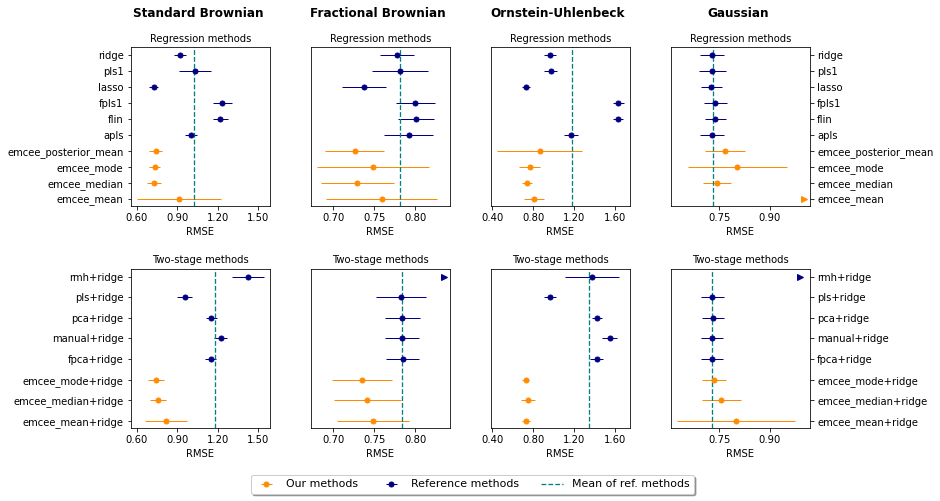
\includegraphics[width=.9\textwidth]{reg_emcee_rkhs}
  \caption{Mean and standard error of RMSE of predictors (lower is better) for 10 runs with GP regressors, one in each column, that obey an underlying linear RKHS model. The first row are direct methods and the second are dimensionality reduction methods.}\label{fig:reg_emcee_rkhs}
\end{figure}

In Figure~\ref{fig:reg_emcee_l2} we see the results for the case with an underlying \(L^2\)-model, which would be our most direct competitor. In this case the outcome is satisfactory, since for the most part our models are on a par with the rest, even beating other methods that were designed with the \(L^2\)-model in mind. Moreover, whenever one of our models has a higher RMSE, the difference is pretty small in comparison. Note that some of our Bayesian models have a higher standard deviation, partly because there is an intrinsic randomness in the methods, and it can be the cause of the occasional worse performance. In relation to this, we observe that the methods that use the mean as a summary statistic tend to perform much worse. Since the mean is very sensitive to outliers, if at some point a MCMC chain randomly deviates from the rest, the average of the posterior samples is greatly impacted.

\begin{figure}[ht!]
  \centering
  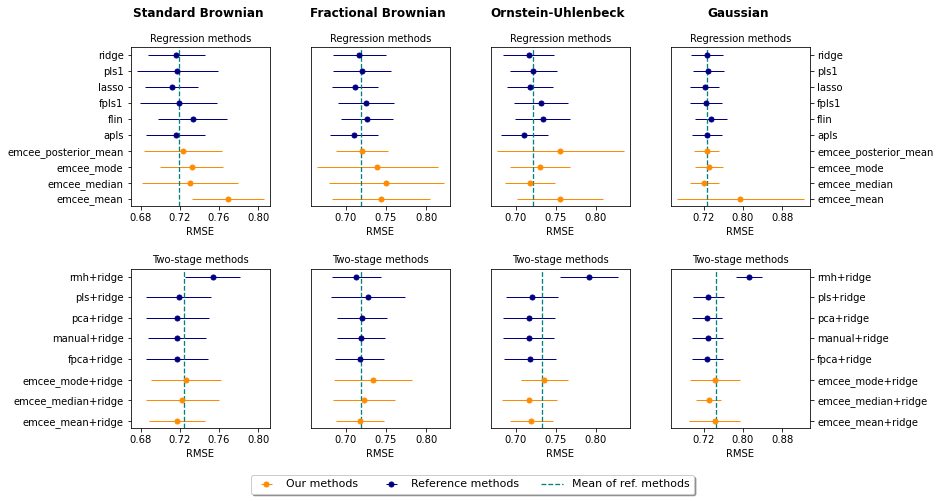
\includegraphics[width=.9\textwidth]{reg_emcee_l2}
  \caption{Mean and standard error of RMSE of predictors (lower is better) for 10 runs with GP regressors, one in each column, that obey an underlying linear \(L^2\)-model. The first row are direct methods and the second are dimensionality reduction methods.}\label{fig:reg_emcee_l2}
\end{figure}

\subsubsection*{Real data}

Figure~\ref{fig:reg_emcee_real} shows the results for the real data sets, where we can see that there is sometimes a substantial difference in performance between some of our methods and the reference algorithms. However, our predict-then-summarize approach (\textit{emcee\_posterior\_mean}) seems to work quite well, always scoring near the mean RMSE of all the comparison algorithms. Moreover, our two-stage methods seem to outperform the summarize-then-predict methods in the Moisture and Sugar data sets, scoring again very close to the mean of the reference models. We have to bear in mind that real data is more complex and noisy than simulated data, and it is possible that after a suitable pre-preprocessing we would obtain better results. However, our goal was to perform a general comparison without focusing too much on the specifics of any particular data set.

\begin{figure}[ht!]
  \centering
  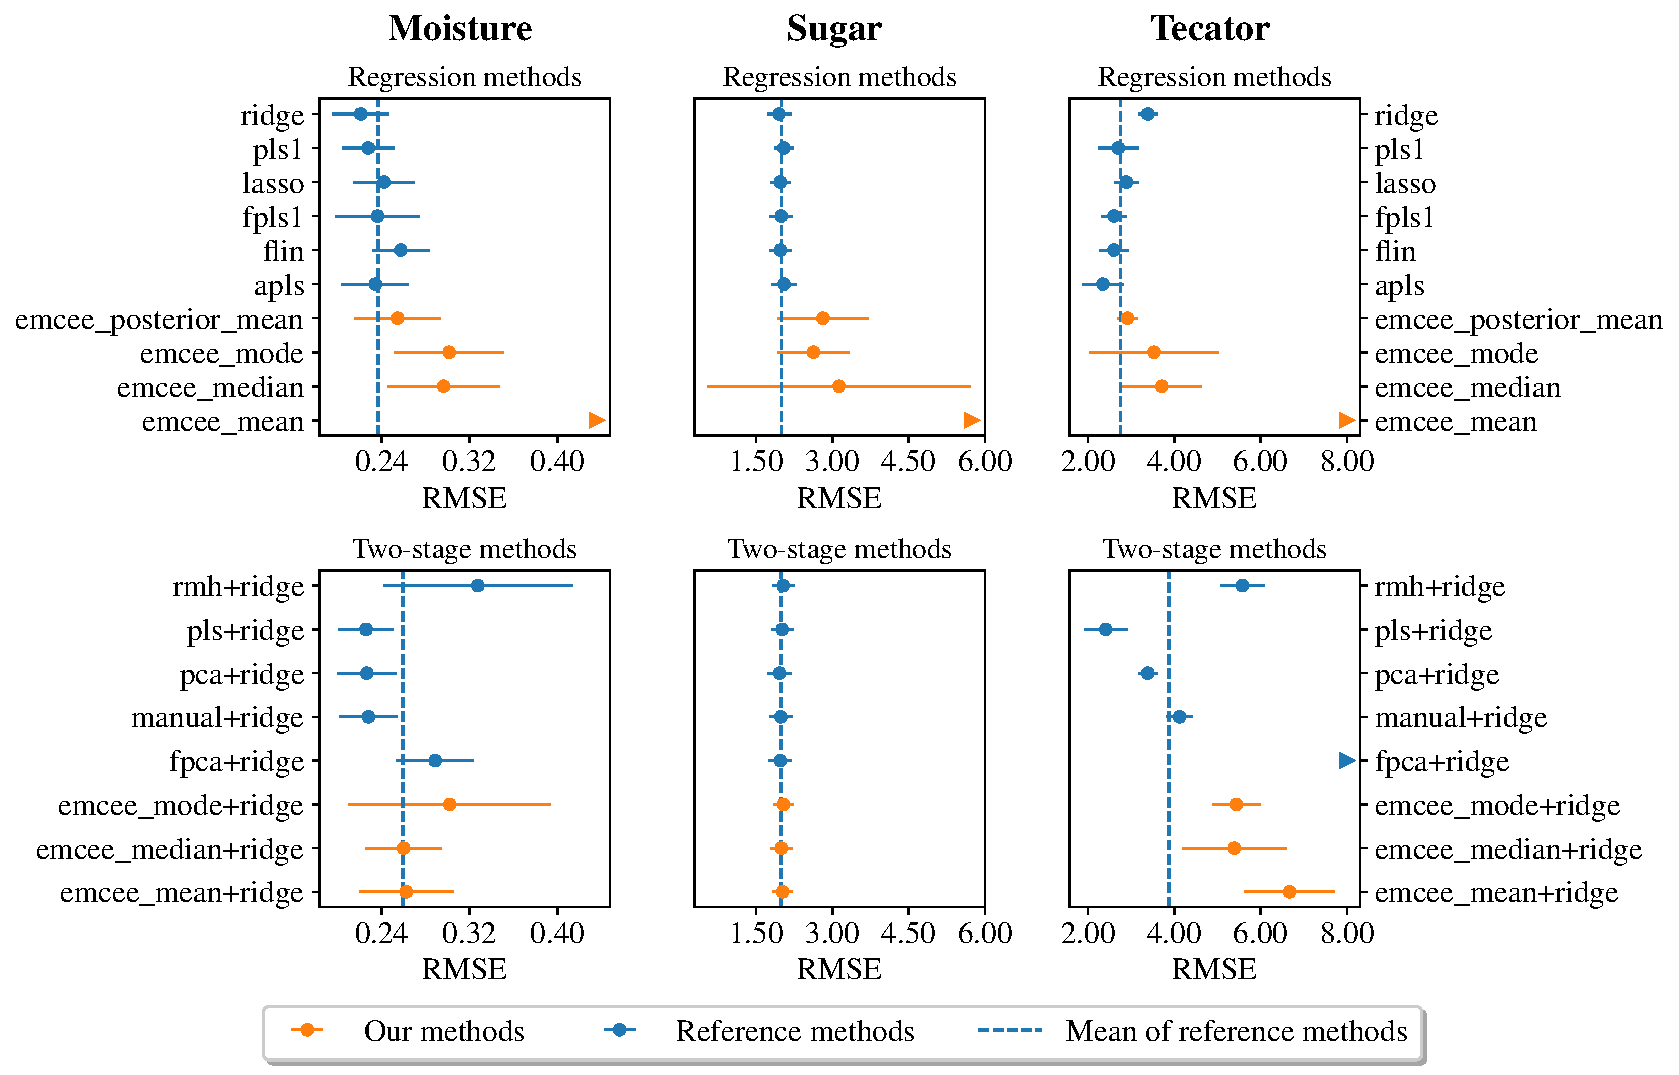
\includegraphics[width=.75\textwidth]{reg_emcee_real}
  \caption{Mean and standard error of RMSE of predictors (lower is better) for 10 runs with real data sets, one in each column. The first row are direct methods and the second are dimensionality reduction methods.}\label{fig:reg_emcee_real}
\end{figure}


\subsection{Functional logistic regression}\label{sec:experiments-logistic}

\subsubsection*{Simulated data sets}

In Figure~\ref{fig:clf_emcee_rkhs} we see the results for the GP regressors in the logistic RKHS case. Our models perform fairly well in this advantageous case, although they are not always better than the comparison methods. However, in most cases the differences observed account for only one or two misclassified samples. 


\begin{figure}[ht!]
  \centering
  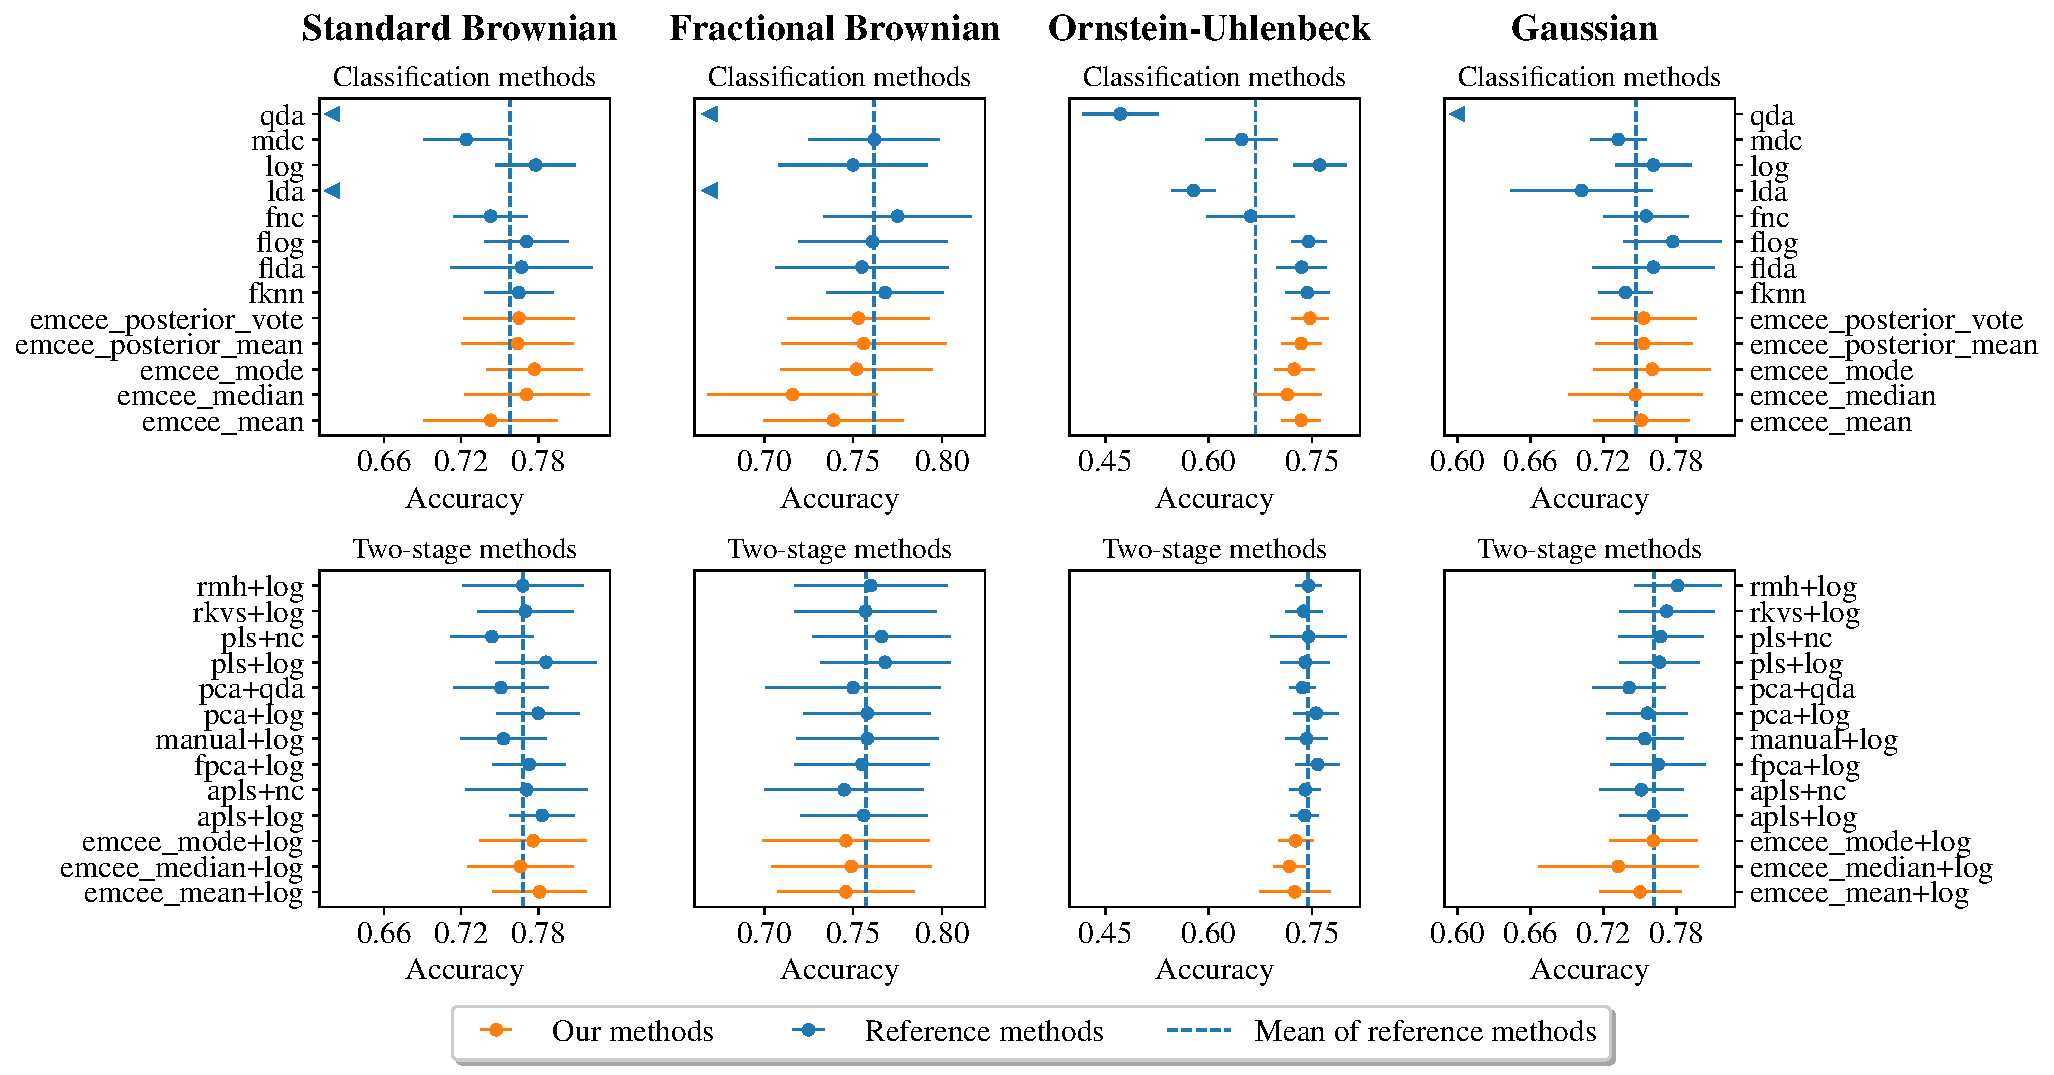
\includegraphics[width=.9\textwidth]{clf_emcee_rkhs}
  \caption{Mean and standard error of accuracy of classifiers (higher is better) for 10 runs with GP regressors, one in each column, that obey an underlying logistic RKHS model. The first row are direct methods and the second are dimensionality reduction methods.}\label{fig:clf_emcee_rkhs}
\end{figure}

Moreover, Figure~\ref{fig:clf_emcee_l2} shows that the results in the \(L^2\) case are again promising, since our models score consistently on or above the mean of the reference models, and in many instances surpass most of them. The predict-then-summarize approaches (\textit{emcee\_posterior\_mean} and \textit{emcee\_posterior\_vote}) are particularly good in this case, and in general have low standard errors. Moreover, the overall accuracy of all methods is poor (below 60\%), so this is indeed a difficult problem in which even small increases in accuracy are relevant.

\begin{figure}[ht!]
  \centering
  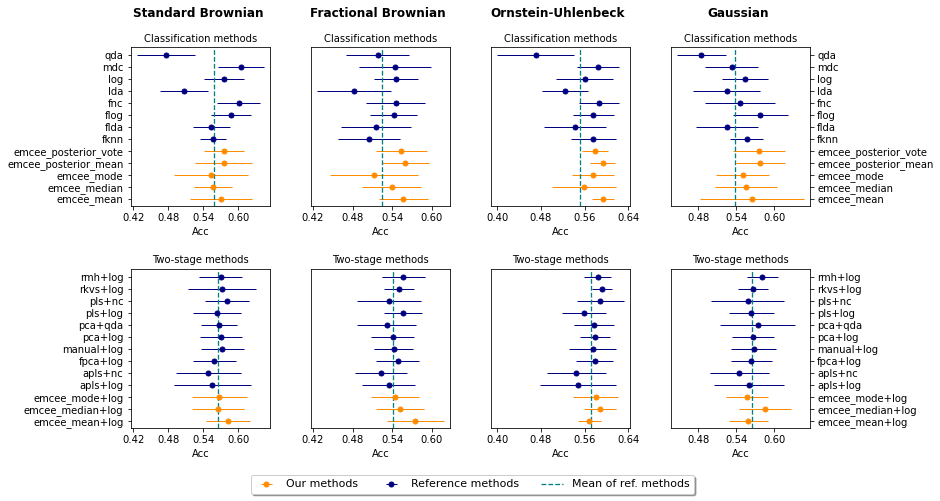
\includegraphics[width=.9\textwidth]{clf_emcee_l2}
  \caption{Mean and standard error of accuracy of classifiers (higher is better) for 10 runs with GP regressors, one in each column, that obey an underlying logistic \(L^2\)-model. The first row are direct methods and the second are dimensionality reduction methods.}\label{fig:clf_emcee_l2}
\end{figure}

\subsubsection*{Real data}

As for the real data sets, in Figure~\ref{fig:clf_emcee_real} we see positive results in general, obtaining in most cases accuracies well above the mean of the reference models, and sometimes above most of them. In particular, the predict-then-summarize methods tend to have a good performance and achieve a lower standard error across executions, which is a trend that we also saw in the simulated data sets. However, as we have been seeing almost invariably, the models that use \textit{emcee\_mean} are the exception: in all these data sets they perform steadily worse than the rest of our Bayesian models. Moreover, we can appreciate that for the most part our logistic models perform better when compared to our linear regression models.

\begin{figure}[ht!]
  \centering
  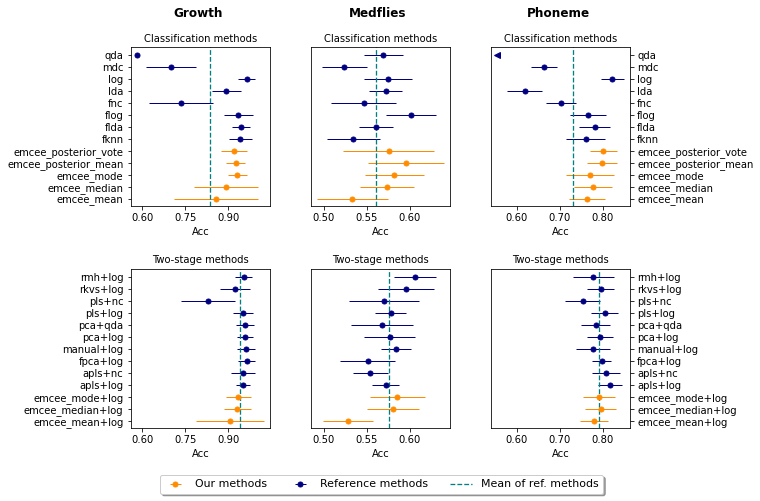
\includegraphics[width=.75\textwidth]{clf_emcee_real}
  \caption{Mean and standard error of accuracy of classifiers (higher is better) for 10 runs with real data sets, one in each column. The first row are direct methods and the second are dimensionality reduction methods.}\label{fig:clf_emcee_real}
\end{figure}


\section{Conclusion}\label{sec:conclusion}

In this work we have introduced a natural and computationally feasible way of integrating Bayesian inference into functional regression models, by means of a RKHS approach that simplifies the usually hard task of setting a prior distribution on a functional space. Moreover, the RKHS framework motivates models based on a linear combination of marginals of the underlying stochastic process, which in a way gives a theoretical background to these popular models, but still retains the functional point of view. Our finite-dimensional approximation has the advantage of working with simpler functional parameters, thus increasing the interpretability and ease of implementation. In addition, it is worth pointing out that our approach works especially well in the logistic case, bypassing the difficulties associated with maximum likelihood techniques and providing a tractable alternative to the more studied methods in the literature.

We have also proved a posterior consistency result that ensures the coherence and correctness of the Bayesian methods we developed. These kinds of results have in other contexts more intricate and restrictive conditions to arrive at essentially the same conclusions as we did, but again the introduction of RKHS's is the key point to greatly simplifying them. In the end, we can regard our derivations as yet another way of applying the abstract posterior consistency theorem of Doob to a concrete situation, giving a positive answer to a problem which was not originally envisioned by this result. Lastly, we have presented numerical evidence that supports the proposed RKHS-based Bayesian methodology and its predictive performance with simulated and real data. This practical side of our work goes to show that the prediction methods we constructed from the posterior distribution are competitive against several non-cherry-picked frequentist alternatives, while still remaining relatively simple, interpretable and viable implementation-wise.



%%%%%%%%%%%%%%%%%%%%%%%%%%%%%%%%%%%%%%%%%%%%%%%%%%%%%%%%%%%%%%%%%%%%%%%%%%
%% Acknowledgments
%%%%%%%%%%%%%%%%%%%%%%%%%%%%%%%%%%%%%%%%%%%%%%%%%%%%%%%%%%%%%%%%%%%%%%%%%%

{\footnotesize
\subsubsection*{Acknowledgments}
  This research was partially supported by grants PID2019-109387GB-I00 and PRE2020-095147 of the Spanish Ministry of Science and Innovation (MCIN), co-financed by the European Social Fund (ESF). J. R. Berrendero and A. Cuevas acknowledge financial support from grant CEX2019-000904-S funded by MCIN/AEI/ 10.13039/501100011033. The authors also wish to acknowledge the computational resources provided by the Centro de Computación Científica-Universidad Autónoma de Madrid (CCC-UAM).
}



%%%%%%%%%%%%%%%%%%%%%%%%%%%%%%%%%%%%%%%%%%%%%%%%%%%%%%%%%%%%%%%%%%%%%%%%%%
%% References
%%%%%%%%%%%%%%%%%%%%%%%%%%%%%%%%%%%%%%%%%%%%%%%%%%%%%%%%%%%%%%%%%%%%%%%%%%

\bibliography{bibliography}



%%%%%%%%%%%%%%%%%%%%%%%%%%%%%%%%%%%%%%%%%%%%%%%%%%%%%%%%%%%%%%%%%%%%%%%%%%
%% Appendices
%%%%%%%%%%%%%%%%%%%%%%%%%%%%%%%%%%%%%%%%%%%%%%%%%%%%%%%%%%%%%%%%%%%%%%%%%%

\newpage
\appendix
%%%%%%%%%%%%%%%%%%%%%%%%%%%%%%%%%%%%%%%%%%%%%%%%%%%%%%%%%%%%%%%%%%%%%%%%
% Copyright (c) 2023 The authors
%
% This work is licensed under a
% Creative Commons Attribution-ShareAlike 4.0 International License.
%
% You should have received a copy of the license along with this
% work. If not, see <http://creativecommons.org/licenses/by-sa/4.0/>.
%%%%%%%%%%%%%%%%%%%%%%%%%%%%%%%%%%%%%%%%%%%%%%%%%%%%%%%%%%%%%%%%%%%%%%%%


%%%%%%%%%%%%%%%%%%%%%%%%%%%%%%%%%%%%%%%%%%%%%%%%%%%%%%%%%%%%%%%%%%%%%%%%%%
%% Supplementary material
%%%%%%%%%%%%%%%%%%%%%%%%%%%%%%%%%%%%%%%%%%%%%%%%%%%%%%%%%%%%%%%%%%%%%%%%%%

\section{Model choice and implementation details}

\subsection{Label switching}\label{app:label-switching}

A well-known issue that arises when using MCMC methods in mixture-like models such as the one proposed in this work is \textit{label switching}, which in short refers to the non-identifiability of the components of the model caused by their interchangeability. In our case, this happens because the likelihood is symmetric with respect to the ordering of the component parameters \(b\) and \(\tau\), that is, \(\pi(Y|X,\theta)=\pi(Y|X, \nu(\theta))\) for any permutation \(\nu\) that rearranges the indices \(j=1,\dots, p\). Thus, since the components are arbitrarily ordered, they may be inadvertently exchanged from one iteration to the next in a MCMC algorithm. This can cause nonsensical answers when summarizing the marginal posterior distributions to perform inference, as different labelings might be mixed on each component \citep{stephens2000dealing}. However, this phenomenon is perhaps surprisingly a condition for the convergence of the MCMC method: as pointed out by many authors \citep[e.g.][]{celeux2000computational}, a lack of switching would indicate that not all modes of the posterior distribution were being explored by the sampler. For this reason, many ad-hoc solutions revolve around post-processing and relabeling the samples to eliminate the switching effect, but they generally do not prevent it from happening in the first place.

The most straightforward solutions consist on imposing an artificial identifiability constraint on the parameters to break the symmetry of their posterior distributions; see \citet{jasra2005markov} and references therein. A common approach that seems to work well is to simply enforce an ordering in the parameters in question, which in our case would mean requiring for example that \(\beta_i < \beta_j\) for \(i < j\), or the analogous with the times in \(\tau\). We have implemented a variation of this method described in \citet{simola2021approximate}, which works by post-processing the samples and relabeling the components to satisfy the order constraint mentioned above, choosing either \(b\) or \(\tau\) depending on which set of ordered parameters would produce the largest separation between any two of them (suitably averaged across all iterations of the chains). This is an area of ongoing research, and thus there are other, more complex relabeling strategies, both deterministic and probabilistic. A summary of several such methods can be found for example in \citet{rodriguez2014label} and \citet{papastamoulis2015label}.

\subsection{Selection of hyperparameters}\label{app:hyperparameters}

One of the key decisions in our Bayesian modeling scheme was whether to consider the number of components \(p\) as a member of the parameter space and integrate it into the model. While theoretically we could impose a prior distribution on \(p\) as well (e.g.\ a categorical distribution with a fixed maximum value), we found that this would have some unwanted practical implications. For instance, it would make the implementation more complex, since the dimensionality of the parameters \(b\) and \(\tau\) would need to be fixed at a certain maximum value beforehand, but the working value of \(p\) within the MCMC algorithm would vary from one iteration to the next. In this case we would have no immediate way of tracking down which set of parameters is ``active'' at any given time. A simple approach would be to always consider the first \(p\) parameters and ignore the rest, and we did indeed try this technique, but it gave rise to new difficulties and the results obtained were not good. In fact, the label switching issue is accentuated when \(p\) is allowed to vary \citep[c.f.][Section~2.3]{grollemund2019bayesian}, and on top of that, the interpretation of, say, the first coefficient \(\beta_1\) in a model with \(3\) components is different from the interpretation of the same coefficient in a model with only \(2\) components.

This inconsistency in the interpretation of the components when the dimensionality of the model increases or decreases could be mitigated using a particular type of MCMC method known as reversible-jump MCMC \citep{green1995reversible}. Theoretically, these algorithms are specifically designed to approximate the posterior distribution in mixture-like models when the number of components is unknown, allowing the underlying dimensionality to change between iterations. However, since they are not yet widely adopted in practice and a reference implementation is not available, we decided against using them in our applications. Another possibility would be to adapt a purely Bayesian model selection technique to our framework \citep[see][]{piironen2017comparison, gelman2013bayesian}, or even derive some model aggregation methods to combine the posterior distributions obtained for different-sized models. These methods are usually based in computing a quantity known as the \textit{Bayes factor}, which in turn requires the specific value of the normalizing integral constant we have been trying to avoid all along. In the end, for the sake of simplicity we decided to let \(p\) be a hyperparameter, so that we could use any model selection criteria (e.g.\ BIC, DIC or cross-validation) to select its optimal value.

As for the default values of the rest of hyperparameters in the prior distributions we propose, several comments are in order:
\begin{itemize}
    \item For the expected value \(b_0\) we propose to use the MLE of \(b\). Although the likelihood function is rather involved, an approximation of the optimal value is enough for our purposes. Our numerical studies suggest that the results are much better with this choice than, say, with a random or null vector.
    \item We found that the parameter \(g\) does not have as much influence on the final result, and the experimentation indicates that \(g=5\) is a good enough value.
    \item Lastly, we observed that the choice of \(\eta\) can have a considerable impact on the final predictors. This is why, in an effort to normalize its scale, we consider a compound parameter \(\eta = \tilde \eta \lambda_{\max}(\mathcal X_\tau^T \mathcal X_\tau)\), where \(\lambda_{\max}(\mathcal X_\tau^T \mathcal X_\tau)\) is the largest eigenvalue of the matrix \(\mathcal X_\tau^T \mathcal X_\tau\), and \(\tilde\eta > 0\) is the actual tuning parameter (which can be selected for instance by cross-validation strategies). This standardization technique has been used previously in the literature; see for example \citet{grollemund2019bayesian}.
\end{itemize}

\subsection{Affine-invariant ensemble sampler}\label{app:ensemble-sampler}

An interesting and often desirable property of MCMC sampling algorithms is that they be \textit{affine-invariant}, which means that they regard two distributions that differ in an affine transformation, say \(\pi(x)\) and \(\pi_{A, b}(Ax + b)\), as equally difficult to sample from. This is useful when one is working with very asymmetrical or skewed distributions, for an affine transformation can turn them into ones with simpler shapes. Generally speaking, a MCMC algorithm can be described through a function \(R\) as \(\Lambda(t+1)=R(\Lambda(t), \xi(t), \pi)\), where \(\Lambda(t)\) is the state of the chain at instant \(t\), \(\pi\) is the objective distribution, and \(\xi(t)\) is a sequence of i.i.d.\ random variables that represent the random behavior of the chain. With this notation, the affine-invariance property can be characterized as \(R(A\lambda+b, \xi(t), \pi_{A,b}) = AR(\lambda, \xi(t), \pi) + b\), for all \(A,b\) and \(\lambda\), and almost all \(\xi(t)\). This means that if we fix a random generator and run the algorithm twice, one time using \(\pi\) and starting in \(\Lambda(0)\) and a second time using \(\pi_{A,b}\) with initial point \(\Gamma(0)=A\Lambda(0)+b\), then \(\Gamma(t)=A\Lambda(t)+b\) for all \(t\). In \citet{goodman2010ensemble} the authors consider an ensemble of samplers with the affine invariance property. Specifically, they work with a set \(\Lambda=(\Lambda_1, \dots, \Lambda_L)\) of \textit{walkers}, where \(\Lambda_l(t)\) represents an individual chain at time \(t\). At each iteration, an affine-invariant transformation is used to find the next point, which is constructed using the current values of the rest of the walkers (similar to Gibb's algorithm), namely the \textit{complementary ensemble}
\[
    \Lambda_{-l}(t) = \{\Lambda_1(t+1), \dots, \Lambda_{l-1}(t+1), \Lambda_{l+1}(t), \dots, \Lambda_L(t)\}, \quad l=1,\dots, L.
\]

To maintain the affine invariance and the joint distribution of the ensemble, the walkers are advanced one by one following a Metropolis-Hastings acceptance scheme. There are mainly two types of moves:

\begin{description}
    \item[Stretch move.]  For each walker \(1\leq l \leq L\) another walker \(\Lambda_j \in \Lambda_{-l}(t)\) is chosen at random, and the proposal is constructed as
        \[
            \Lambda_l(t) \to \Gamma = \Lambda_j + Z(\Lambda_l(t) - \Lambda_j),
        \]
        where \(Z \stackrel{i.i.d.}{\sim} g(z)\) satisfying the symmetry condition \(g(z^{-1})=zg(z)\). In particular, the suggested density is
        \[
            g_a(z) \propto \begin{cases}
                \frac{1}{\sqrt{z}}, & \text{if } z \in [a^{-1}, a], \\
                0,                  & \text{otherwise.}
            \end{cases}, \quad a > 1.
        \]
        Supposing \(\R^p\) is the sample space, the corresponding acceptance probability (chosen so that the detailed balance equations are satisfied) is:
        \[
            \alpha = \min\left\{1, \ Z^{p-1}\frac{\pi(\Gamma)}{\pi(\Lambda_l(t))}\right\}.
        \]

    \item[Walk move.] For each walker \(1\leq l \leq L\) a random subset \(S_l \subseteq \Lambda_{-l}(t)\) with \(|S_l| \geq 2\) is selected, and the proposed move is
        \[
            \Lambda_l(t) \to \Gamma = \Lambda_l(t) + W,
        \]
        where \(W\) is a normal distribution with mean \(0\) and the same covariance as the sample covariance of all walkers in \(S_l\). The acceptance probability in this case is just the Metropolis ratio, that is, \(\alpha=\min\{1, \pi(\Gamma)/\pi(\Lambda_l(t))\}\).
\end{description}

From a computational perspective, the Python library \textit{emcee} \citep{foreman2013emcee} provides a parallel implementation of this algorithm. The idea is to divide the ensemble \(\Lambda\) into two equally-sized subsets \(\Lambda^{(0)}\) and \(\Lambda^{(1)}\), and then proceed on each iteration in the following alternate fashion:
\begin{enumerate}
    \item Update \textit{all} walkers in \(\Lambda^{(0)}\) through one of the available moves explained above, using \(\Lambda^{(1)}\) as the complementary ensemble.
    \item Use the new values in \(\Lambda^{(0)}\) to update \(\Lambda^{(1)}\).
\end{enumerate}
In this way the detailed balance equations are still satisfied, and each of the steps can benefit from the computing power of an arbitrary number of processors (up to \(L/2\)).

\subsection{MCMC implementation}\label{app:mcmc}

The MCMC method chosen for approximating the posterior distribution in our models is the affine-invariant ensemble sampler described in Appendix~\ref{app:ensemble-sampler}. As mentioned there, we utilize the computational implementation in the Python library \textit{emcee}, which is both reliable and easy to use; it aims to be a general-purpose package that performs well in a wide class of problems. One advantage of this method, apart from the property of affine-invariance, is that it only requires us to specify a few hyperparameters, irrespective of the underlying dimension. This contrasts to, say, the \(\mathcal O(N^2)\) degrees of freedom corresponding to the covariance matrix of an \(N\)-dimensional jump distribution in Metropolis-Hastings. After selecting the number of iterations and the number of chains we want, we need to specify the initial points for each of them. As pointed out in \citet{foreman2013emcee}, a good initial choice is a Gaussian ball around a point in \(\Theta_p\) that is expected to have a high probability with respect to the objective distribution. In our implementation we adopt this method, choosing an approximation of the MLE of \(\theta\) as the central point in each case. To perform this approximation we employ the Basin-hopping optimization algorithm \citep{wales1997global}. This is a two-phase stochastic method that combines global steps with local optimization, in the hope of avoiding getting stuck too quickly in local maxima. To reduce the effects of randomness, we run the algorithm a few times and retain the point with the highest likelihood, and to avoid biasing the sampler too much towards the specific point selected, we let a fraction of the initial points be random (within reasonable bounds). This approximation is also used to specify the hyperparameter \(b_0\).

Other less relevant hyperparameters include the burn-in period for the chains, which is the number of initial samples discarded, or the amount of thinning performed, which is the number of consecutive samples discarded to reduce the correlation among them. We use 64 chains and run them for 900 iterations in total, discarding the first 500 iterations as burn-in. Moreover, we use a weighted mixture of \textit{walk} and \textit{stretch} moves in the \textit{emcee} sampler to advance the chains in each iteration, selecting the stretch move (the default) with probability 0.7 or the walk move with probability 0.3. Another computational decision we made is working with \(\log \sigma\) instead of \(\sigma^2\), so that the domain of this parameter is an unconstrained space, which is a widespread recommendation that helps increase the efficiency of the method.

\newpage
\section{Measure-theoretic subtleties}\label{app:measure-theory}

There are some technicalities to take into account in the theoretical exposition in Section~\ref{sec:consistency}, especially pertaining to measure theory. For example, to justify the existence of regular conditional distributions such as \(\bm\theta|X_1,\dots,X_n\), one should see Theorem 10.2.1 and Theorem 10.2.2 in \citet{dudley2002real}, which guarantee they are well-defined provided that the underlying spaces are sufficiently regular. Another issue is the measurability of the mapping \(\theta \mapsto P_\theta(X,Y)(A)\), which is assumed in the proof of the consistency results. We illustrate how this can be proved for example in the linear case, under the additional condition of sample continuity, which is arguably not a very restrictive condition in real-life scenarios.

\begin{proposition}
    If the process \(X\) is sample-continuous (i.e.\ the trajectories are continuous functions), then the mapping \(\theta \mapsto P_\theta(X,Y)(A)\) is measurable for every measurable set \(A \subseteq \mathcal X \times \mathcal Y\).
\end{proposition}

\begin{proof}
    We start by checking that \(\theta \mapsto P_\theta(Y|X)(A_1)\) is measurable for every measurable set \(A_1\subseteq \mathcal Y\). Indeed, consider the function \(F(y,\theta)=f(y|X,\theta)\bm{1}_{A_1}(y)\), where \(f(\cdot|X,\theta)\) is the density of the normal distribution \(\mathcal N(\alpha_0 + \sum_j \beta_j X(t_j), \sigma^2)\) and \(\bm{1}_A\) is the indicator function of a set \(A\). It is easy to see that \(F(y,\theta)\) is jointly measurable (it is in fact continuous) if \(X\) has continuous sample paths. Then, by Tonelli's theorem \citep[e.g.][Theorem~2.37]{folland1999real}, the function
    \[
        \theta \mapsto \int_{\mathcal Y} f(y|X,\theta)\bm{1}_{A_1}(y)\, dy = \E_{P_\theta(Y|X)}\left[\bm{1}_{A_1}(Y)\right] = P_\theta(Y|X)(A_1)
    \]
    is measurable. Now, if \(A\) is a measurable subset of \(\mathcal X \times \mathcal Y\), we have
    \[
        P_\theta(X,Y)(A)  = \int_{\mathcal X} P_\theta(Y|X=x)(A_x) dP(X)(x),
    \]
    where \(A_x=\{y\in\mathcal Y: (x,y) \in A\}\) is the \(x\)-section of \(A\). We just saw that \(\theta \mapsto P_\theta(Y|X=x)(A_x)\) is measurable, and thus we conclude that \(\theta \mapsto P_\theta(X,Y)(A)\) is measurable, since integration respects measurability.
\end{proof}

\newpage
\section{Experimentation}\label{app:experimentation}

\subsection{Overview of data sets and comparison algorithms}\label{app:data-sets}

To generate the simulated data sets for the comparison experiments of Section~\ref{sec:results}, we used four types of Gaussian process regressors commonly employed in the literature, each with a different covariance function:
\begin{description}
    \item [BM.] A Brownian motion, with kernel \(K_1(t,s)=\min\{t,s\}\).
    \item [fBM.] A fractional Brownian motion, with kernel \(K_2(t,s)=1/2(s^{2H} + t^{2H} - |t-s|^{2H})\) and Hurst parameter \(H=0.8\).
    \item [O-U.] An Ornstein-Uhlenbeck process, with kernel \(K_3(t,s)=e^{-|t-s|}\).
    \item [Gaussian.] A Gaussian process with Gaussian kernel \(K_4(t,s)=e^{-(t-s)^2/2\nu^2}\), where \(\nu=0.2\).
\end{description}

For the comparison algorithms themselves, we considered several frequentist methods which were selected among popular ones in FDA and machine learning in general. As was specified in Section~\ref{sec:results}, variable selection and dimensionality reduction methods are part of a pipeline followed by a standard multiple regression technique. In the linear regression case, we chose the following algorithms:

\begin{description}
    \item[Manual.] Dummy variable selection method with a pre-specified number of components (equispaced on \([0, 1]\)).
    \item[Lasso] Linear least squares with \(l^1\) regularization.
    \item [Ridge.] Linear least squares with \(l^2\) regularization.
    \item [PLS.] Partial least squares for dimension reduction.
    \item [PCA.] Principal component analysis for dimension reduction.
    \item [PLS1.] Partial least squares regression \citep[e.g.][]{abdi2010partial}.
    \item [APLS.] Functional partial least squares regression proposed by \citet{delaigle2012methodology}.
    \item [RMH.] Recursive maxima hunting variable selection method proposed by \citet{torrecilla2016feature}.
    \item [FLin.] Functional \(L^2\) linear regression model with fixed basis expansion.
    \item [FPCA.] Functional principal component analysis.
    \item [FPLS1.] Functional PLS regression through basis expansion, implemented as in \citet{aguilera2010using}.
\end{description}
In the logistic regression case, all the variable selection and dimension reduction techniques from above were also considered, with the addition of the following classification methods:
\begin{description}
    \item [Log.] Standard multiple logistic regression with \(l^2\) regularization.
    \item [LDA.] Linear discriminant analysis.
    \item [QDA.] Quadratic discriminant analysis.
    \item [RKVS.] RKHS-based variable selection and classification method proposed in \citet{berrendero2018use}.
    \item [APLS.] Functional PLS used as a dimension reduction method, as proposed in \citet{delaigle2012achieving} in combination with the nearest centroid (NC) algorithm.
    \item [FLog.] Functional RKHS-based logistic regression algorithm proposed in \citet{berrendero2023functional}.
    \item [FLDA.] Implementation of the functional version of linear discriminant analysis proposed in \citet{preda2007pls}.
    \item [MDC.] Maximum depth classifier \citep[e.g.][]{ghosh2005maximum}.
    \item [FKNN.] Functional K-nearest neighbors classifier with the \(L^2\)-distance.
    \item [FNC.] Functional nearest centroid classifier with the \(L^2\)-distance.
\end{description}

The main parameters of all these algorithms are selected by cross-validation, using the same 5 folds as our proposed models so that the comparisons are fair. In particular, regularization parameters are searched among 20 values in the logarithmic space \([10^{-4}, 10^4]\), the number of manually selected variables is one of \(\{5, 10, 15, 20, 25, 50\}\), the number of components for dimension reduction and variable selection techniques is in the set \(\{2, 3, 4, 5, 7, 10, 15, 20\}\), the number of basis elements for cubic spline bases is in \(\{8,10,12,14,16\}\), the number of basis elements for Fourier bases is one of \(\{3,5,7,9,11\}\), and the number of neighbors in the KNN classifier is in \(\{3,5,7,9,11\}\). Most algorithms have been taken from the libraries \textit{scikit-learn} \citep{pedregosa2011scikit} and \textit{scikit-fda} \citep{ramos2023scikit}, the first oriented to machine learning in general and the second to FDA in particular. However, some methods were not found in these packages and had to be implemented from scratch. This is the case of the FLDA, FPLS and APLS methods, which we coded following the corresponding articles.

\subsection{Simulations with non-Gaussian regressors}\label{app:non-gp}

We performed a set of experiments in linear and logistic regression in which the regressors are not Gaussian processes (GPs). These experiments where run in the same conditions as those reported in Section~\ref{sec:results}.

\subsubsection*{Functional linear regression}

We use a geometric Brownian motion (GBM) as the regressor variable, defined as \(X(t)=e^{BM(t)}\), where \(BM(t)\) is a standard Brownian motion. In this case we consider two data sets, one with a RKHS response and one with an \(L^2\) response, both with the same parameters as in the corresponding data sets in Section~\ref{sec:results}. The comparison results can be seen in Figure~\ref{fig:reg_emcee_nongp}: in this case we still get better results under the RKHS model, while the results under the \(L^2\)-model are slightly worse. However, as with other simulations, the difference is small (except for the \textit{emcee\_mean} methods).

\begin{figure}[ht!]
    \centering
    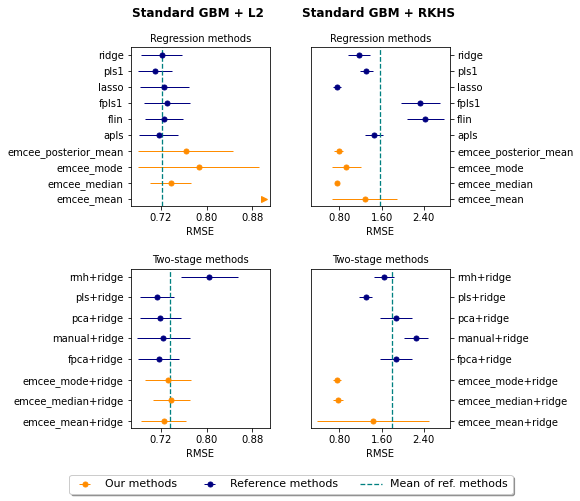
\includegraphics[width=.6\textwidth]{reg_emcee_nongp}
    \caption{Mean and standard error of RMSE of predictors (lower is better) for 10 runs with GBM regressors. In the first column the response obeys a linear \(L^2\)-model, while in the second columns it follows a RKHS linear model. The first row are direct methods and the second are dimensionality reduction methods.}\label{fig:reg_emcee_nongp}
\end{figure}

\subsubsection*{Functional logistic regression}

We consider a ``mixture'' situation in which we combine regressors from two different GPs with equal probability and label them according to their origin. Firstly, we consider a homoscedastic case to distinguish between a standard Brownian motion and a Brownian motion with a mean function that is zero until \(t=0.5\), and then becomes \(m(t)=0.75t\). Secondly, we consider a heteroscedastic case to distinguish between a standard Brownian motion and a Brownian motion with variance 2, that is, with kernel \(K(t,s)=2\min\{t,s\}\). Figure~\ref{fig:clf_emcee_nongp} shows that our classifiers perform better than most comparison algorithms when separating two homoscedastic Gaussian processes, but they struggle in the heteroscedastic case. Incidentally, this heteroscedastic case of two zero-mean Brownian motions has a special interest, since it can be shown that the Bayes error is zero in the limit of dense monitoring (i.e.\ with an arbitrarily fine measurement grid), a manifestation of the ``near-perfect'' classification phenomenon analyzed for example in \citet{torrecilla2020optimal}. Our results are in line with the empirical studies of this article, where the authors conclude that even though the asymptotic theoretical error is zero, most classification methods are suboptimal in practice (possibly due to the high collinearity of the data), with the notable exception of PCA+QDA.

\begin{figure}[ht!]
    \centering
    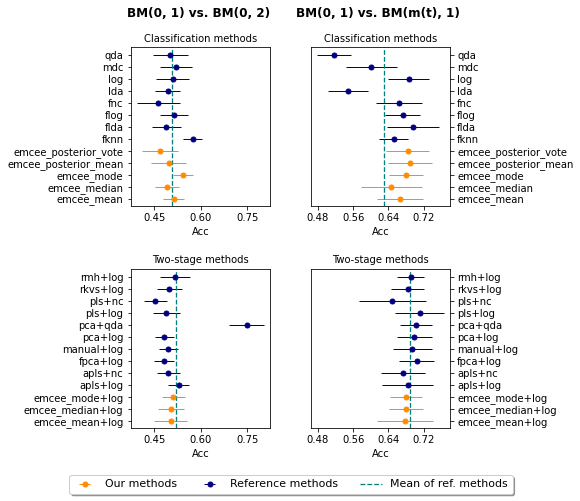
\includegraphics[width=.6\textwidth]{clf_emcee_nongp}
    \caption{Mean and standard error of accuracy of classifiers (higher is better) for 10 runs with a mix of regressors coming from two different GPs and labeled according to their origin. In the first column we try to separate two Brownian motions with the same mean but different variance, while in the second column we discriminate between two Brownian motions with different mean functions but the same variance. The first row are direct methods and the second are dimensionality reduction methods.}\label{fig:clf_emcee_nongp}
\end{figure}

\subsection{Model misspecification}

One requirement that our model should satisfy is that it ought to be able to recover the true parameter function when the underlying data generation model is a finite-dimensional RKHS model. This is generally the case when the value of \(p\) in our model and the true value \(p_0\) coincide, but what happens when we change the value of \(p\) in the model? Take for example a RKHS data set with two components generated according to the formula \(Y=5 -5X(0.1) + 10X(0.8) + \epsilon\), with \(\epsilon\sim \mathcal N(0, 0.5)\). Figure~\ref{fig:beta_trace_3} shows the resulting posterior distribution of the parameters \(b=(\beta_1, \beta_2, \beta_3)\) and \(\tau=(t_1, t_2, t_3)\) for a model with 3 components. As we can see, one of the coefficients has gone to zero to account for the overspecification of the model, while the other two have stabilized very close to the true parameters. The same goes for the time instants, except that in this case there is no default value to represent that a component is unused, so the time corresponding to the null coefficient oscillates back and forth. Note that the estimated function (based for example in the mode of the posterior distributions) will not be perfect, essentially because of the noise in the response. But it should be close to the true parameter function \(\alpha(t)=-5K(t, 0.1) + 10K(t, 0.8)\), providing a good predictive performance in most cases.

\begin{figure}[ht!]
    \centering
    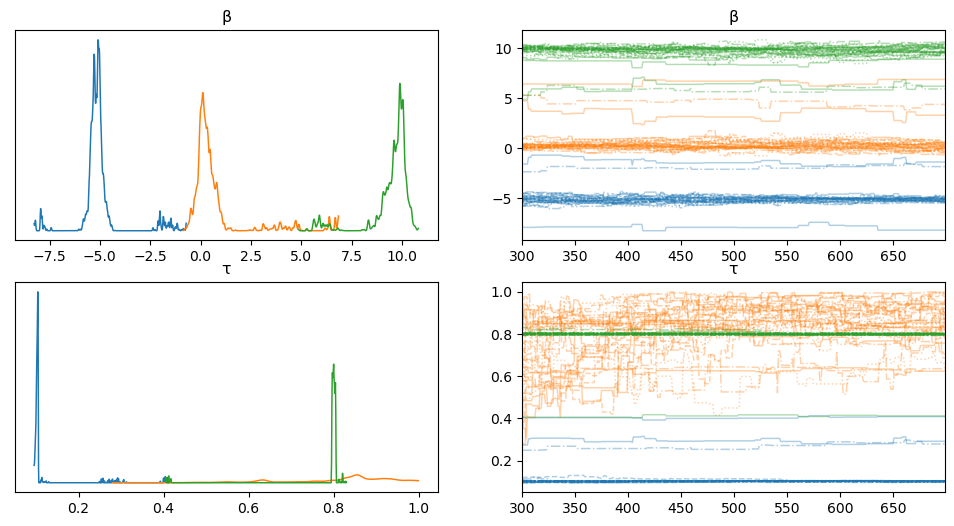
\includegraphics[width=.8\textwidth]{beta_trace_3}
    \caption{Left: estimated posterior distribution for the parameters \(b\) and \(\tau\) using our RKHS linear regression model with \(p=3\), in a linear dataset with \(p_0=2\) components. Right: the corresponding trace evolution for 400 iterations in the MCMC sampler.}\label{fig:beta_trace_3}
\end{figure}

In contrast, if we consider now a model with \(p=4\) with the same data, we might obtain posterior distributions like the ones in Figure~\ref{fig:beta_trace_4}. In this situation two coefficients should go to zero, but that is no longer the case. For example, while the green component has a high density around 0, it also has a considerable mass around 10, effectively ``competing'' with the red component. This is a manifestation of the label switching issue, caused in this case by an excessive number of degrees of freedom in the model. There is still another possible situation, one in which no label switching occurs but the estimated function has four non-negligible components. This can happen because the different components exploit the additional freedom and ``work together'', so to speak. In this way we might obtain an estimate that does not resemble the true coefficient function, but that has a very low prediction error. However, this could also work to our detriment and cause the estimated function to be worse prediction-wise than simpler alternatives. This phenomenon is expected to strengthen as the difference between the true and assumed value of \(p\) grows larger.

\begin{figure}[ht!]
    \centering
    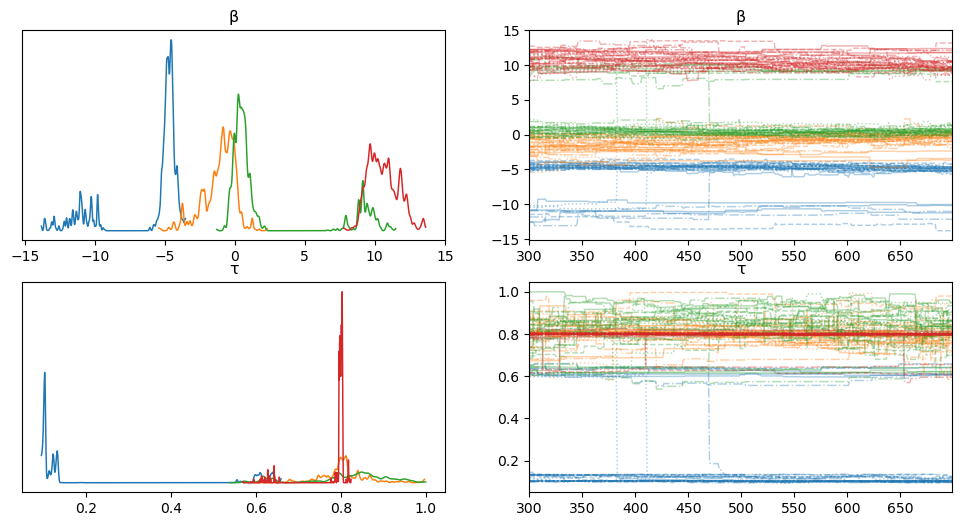
\includegraphics[width=.8\textwidth]{beta_trace_4}
    \caption{Left: estimated posterior distribution for the parameters \(b\) and \(\tau\) using our RKHS linear regression model with \(p=4\), in a linear dataset with \(p_0=2\) components. Right: the corresponding trace evolution for 400 iterations in the MCMC sampler.}\label{fig:beta_trace_4}
\end{figure}

\subsection{Dependence on the number of components}

Another thing we wanted to look at was the dependence of the final prediction result on the chosen value of \(p\), especially when there is no concept of ``components'' in the underlying model. We can take for example the homoscedastic mixture data set described in Appendix~\ref{app:non-gp} for the logistic regression problem, and fix the parameter \(\eta=0.01\). The corresponding mean accuracies (in 10 repetitions) for RKHS models with \(p=1,2,\dots 10\) components are shown in Figure~\ref{fig:dependence_acc_p}, along with their standard errors (which are arguably not very informative). It would appear that the methods that use the whole posterior distribution (\textit{emcee\_posterior\_mean} and \textit{emcee\_posterior\_vote}) are more stable and somewhat independent of the value of \(p>1\) in terms of accuracy. On the other hand, the rest of the algorithms show a slight downward trend as \(p\) increases (although not so much in the variable selection methods), and in general their best results are obtained at \(p=2\). We expect that this effect or some small variation of it will remain valid in other situations, and it would be in line with our view that the RKHS models work best with fewer components. However, a profound study of this would be the subject of a different experiment altogether.

\begin{figure}[ht!]
    \centering
    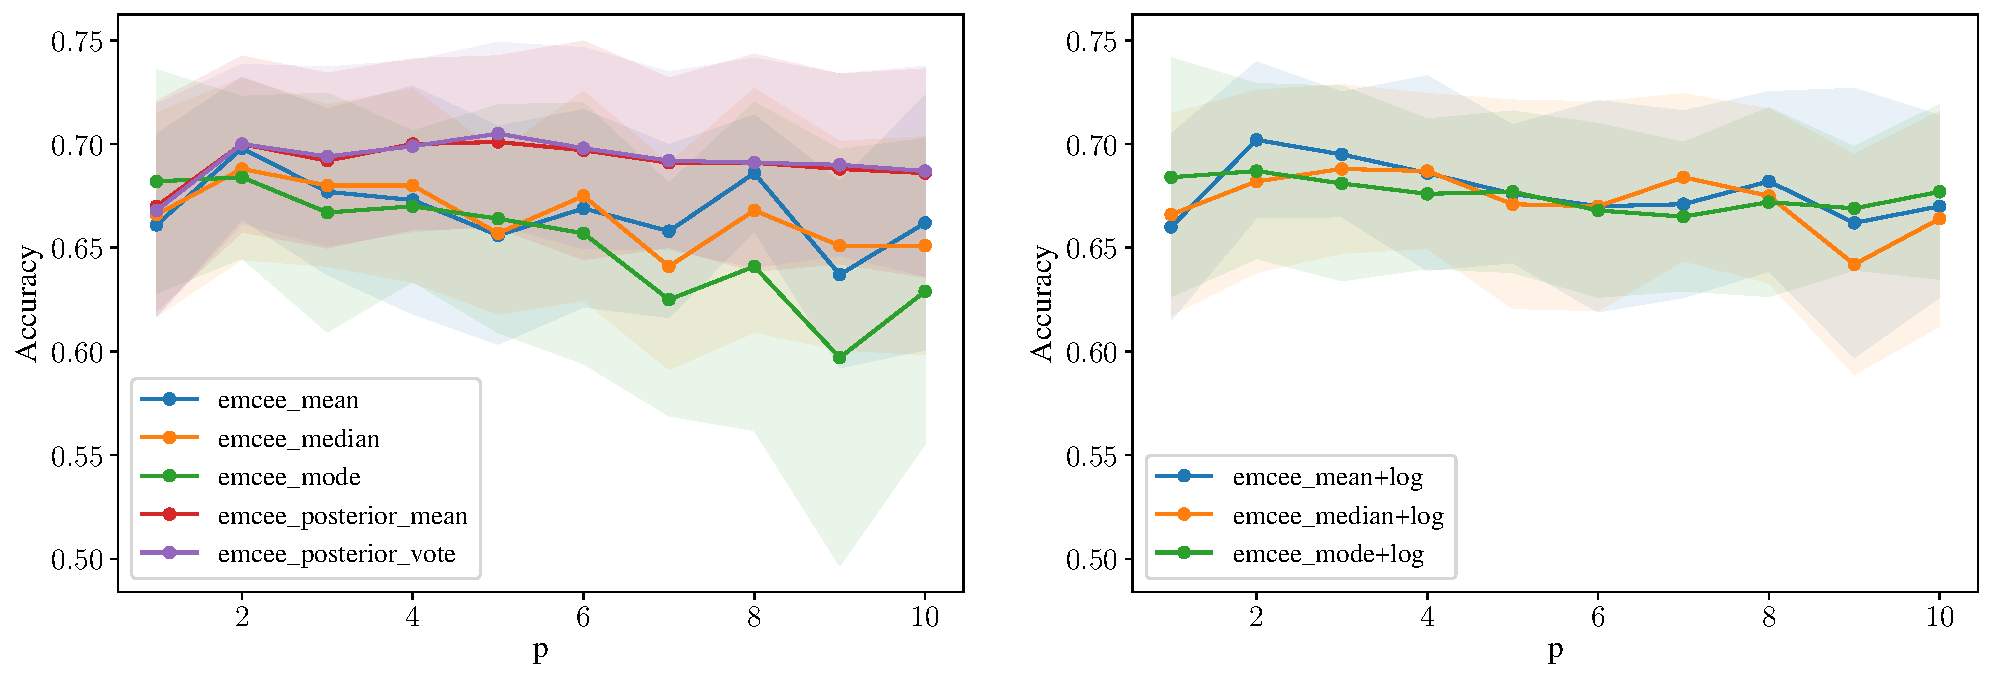
\includegraphics[width=0.85\textwidth]{mixture_dependence_acc_p}
    \caption{Mean accuracy in 10 independent repetitions for our logistic RKHS methods as a function of \(p\), using \(\eta=0.01\) and the homoscedastic mixture data set. The corresponding standard errors are shown in faded colors.}\label{fig:dependence_acc_p}
\end{figure}


\subsection{Tables of experimental results}\label{app:tables}

We present below the tables corresponding to the empirical comparison studies in Appendix~\ref{app:non-gp} and in Section~\ref{sec:results}, which show the numerical values that were depicted there graphically. In each case the best and second-best results are shown in \firstcolor{bold} and \secondcolor{italics}, respectively.

\subsubsection*{Functional linear regression}

\begin{table}[htbp!]
    \footnotesize
    \centering
    \rowcolors{2}{}{teal!8}
    \begin{tabular}{lcccc}
        \toprule
        \textbf{Prediction method} & \textbf{BM}                 & \textbf{fBM}                & \textbf{O-U}                & \textbf{Gaussian}           \\
        \midrule
        emcee\_mean                & 0.913 (0.310)               & 0.759 (0.068)               & 0.806 (0.098)               & 1.408 (1.359)               \\
        emcee\_median              & \secondcolor{0.729 (0.048)} & \secondcolor{0.729 (0.045)} & \secondcolor{0.740 (0.052)} & 0.743 (0.041)               \\
        emcee\_mode                & 0.735 (0.039)               & 0.748 (0.068)               & 0.769 (0.102)               & 0.803 (0.147)               \\
        emcee\_posterior\_mean     & 0.743 (0.047)               & \firstcolor{0.726 (0.036)}  & 0.863 (0.416)               & 0.766 (0.061)               \\
        apls                       & 1.003 (0.045)               & 0.792 (0.030)               & 1.167 (0.068)               & \secondcolor{0.728 (0.035)} \\
        flin                       & 1.219 (0.056)               & 0.800 (0.022)               & 1.630 (0.051)               & 0.738 (0.030)               \\
        fpls1                      & 1.235 (0.069)               & 0.800 (0.024)               & 1.631 (0.053)               & 0.738 (0.035)               \\
        lasso                      & \firstcolor{0.727 (0.034)}  & 0.738 (0.027)               & \firstcolor{0.731 (0.039)}  & \firstcolor{0.726 (0.032)}  \\
        pls1                       & 1.032 (0.116)               & 0.782 (0.034)               & 0.974 (0.063)               & 0.729 (0.041)               \\
        ridge                      & 0.920 (0.043)               & 0.778 (0.021)               & 0.965 (0.059)               & \secondcolor{0.728 (0.035)} \\

        \bottomrule
        \toprule

        emcee\_mean+ridge          & 0.816 (0.154)               & 0.749 (0.044)               & \secondcolor{0.734 (0.039)} & 0.799 (0.175)               \\
        emcee\_median+ridge        & \secondcolor{0.759 (0.063)} & \secondcolor{0.741 (0.041)} & 0.751 (0.065)               & 0.755 (0.058)               \\
        emcee\_mode+ridge          & \firstcolor{0.746 (0.058)}  & \firstcolor{0.735 (0.036)}  & \firstcolor{0.726 (0.038)}  & 0.735 (0.036)               \\
        fpca+ridge                 & 1.149 (0.041)               & 0.784 (0.020)               & 1.420 (0.063)               & \secondcolor{0.728 (0.033)} \\
        manual+ridge               & 1.221 (0.050)               & 0.784 (0.021)               & 1.548 (0.072)               & \firstcolor{0.727 (0.032)}  \\
        pca+ridge                  & 1.153 (0.041)               & 0.784 (0.022)               & 1.422 (0.050)               & 0.730 (0.033)               \\
        pls+ridge                  & 0.955 (0.053)               & 0.783 (0.031)               & 0.962 (0.059)               & 0.729 (0.035)               \\
        rmh+ridge                  & 1.423 (0.117)               & 0.847 (0.043)               & 1.375 (0.266)               & 1.226 (0.117)               \\

        \bottomrule
    \end{tabular}
    \caption{Mean RMSE of predictors (lower is better) for 10 runs with GP regressors, one in each column, that obey an underlying linear RKHS model. The corresponding standard errors are shown between brackets.}
\end{table}
\newpage
\FloatBarrier{}

\begin{table}[htbp!]
    \vspace{.5em}
    \footnotesize
    \centering
    \rowcolors{2}{}{teal!8}
    \begin{tabular}{lcccc}
        \toprule
        \textbf{Prediction method} & \textbf{BM}                 & \textbf{fBM}                & \textbf{O-U}                & \textbf{Gaussian}           \\
        \midrule
        emcee\_mean                & 0.769 (0.037)               & 0.744 (0.061)               & 0.756 (0.054)               & 0.794 (0.129)               \\
        emcee\_median              & 0.730 (0.049)               & 0.751 (0.071)               & 0.718 (0.031)               & \firstcolor{0.722 (0.030)}  \\
        emcee\_mode                & 0.732 (0.032)               & 0.739 (0.075)               & 0.730 (0.038)               & 0.730 (0.029)               \\
        emcee\_posterior\_mean     & 0.723 (0.040)               & 0.720 (0.032)               & 0.755 (0.079)               & \secondcolor{0.726 (0.026)} \\
        apls                       & \secondcolor{0.715 (0.030)} & \firstcolor{0.710 (0.030)}  & \firstcolor{0.710 (0.029)}  & \secondcolor{0.726 (0.031)} \\
        flin                       & 0.733 (0.035)               & 0.727 (0.033)               & 0.733 (0.035)               & 0.735 (0.032)               \\
        fpls1                      & 0.718 (0.039)               & 0.726 (0.035)               & 0.731 (0.034)               & \secondcolor{0.726 (0.033)} \\
        lasso                      & \firstcolor{0.712 (0.027)}  & \secondcolor{0.712 (0.028)} & 0.717 (0.029)               & \firstcolor{0.722 (0.029)}  \\
        pls1                       & 0.717 (0.041)               & 0.720 (0.036)               & 0.722 (0.029)               & 0.729 (0.031)               \\
        ridge                      & 0.716 (0.029)               & 0.717 (0.032)               & \secondcolor{0.716 (0.032)} & 0.727 (0.033)               \\
        \bottomrule
        \toprule
        emcee\_mean+ridge          & \firstcolor{0.717 (0.029)}  & \secondcolor{0.718 (0.030)} & 0.719 (0.027)               & 0.743 (0.052)               \\
        emcee\_median+ridge        & 0.722 (0.038)               & 0.723 (0.038)               & \secondcolor{0.717 (0.035)} & 0.730 (0.025)               \\
        emcee\_mode+ridge          & 0.726 (0.036)               & 0.735 (0.048)               & 0.736 (0.030)               & 0.743 (0.050)               \\
        fpca+ridge                 & \firstcolor{0.717 (0.032)}  & \secondcolor{0.718 (0.030)} & 0.718 (0.033)               & \firstcolor{0.727 (0.031)}  \\
        manual+ridge               & \firstcolor{0.717 (0.030)}  & 0.719 (0.030)               & \firstcolor{0.716 (0.032)}  & \secondcolor{0.728 (0.031)} \\
        pca+ridge                  & \firstcolor{0.717 (0.032)}  & 0.720 (0.031)               & \firstcolor{0.716 (0.032)}  & \firstcolor{0.727 (0.031)}  \\
        pls+ridge                  & \secondcolor{0.719 (0.033)} & 0.728 (0.046)               & 0.720 (0.033)               & 0.730 (0.031)               \\
        rmh+ridge                  & 0.753 (0.029)               & \firstcolor{0.713 (0.030)}  & 0.791 (0.037)               & 0.812 (0.027)               \\
        \bottomrule
    \end{tabular}
    \caption{Mean RMSE of predictors (lower is better) for 10 runs with GP regressors, one in each column, that obey an underlying linear \(L^2\)-model. The corresponding standard errors are shown between brackets.}
\end{table}

\vspace{2em}

\begin{table}[htbp!]
    \footnotesize
    \centering
    \rowcolors{2}{}{teal!8}
    \begin{tabular}{lcc}
        \toprule
        \textbf{Prediction method} & \textbf{GBM + \(\bf{L^2}\)} & \textbf{GBM + RKHS}         \\
        \midrule
        emcee\_mean                & 0.948 (0.354)               & 1.278 (0.622)               \\
        emcee\_median              & 0.737 (0.036)               & \firstcolor{0.747 (0.031)}  \\
        emcee\_mode                & 0.786 (0.106)               & 0.928 (0.275)               \\
        emcee\_posterior\_mean     & 0.763 (0.083)               & 0.786 (0.084)               \\
        apls                       & \secondcolor{0.716 (0.034)} & 1.456 (0.170)               \\
        flin                       & 0.726 (0.033)               & 2.427 (0.352)               \\
        fpls1                      & 0.731 (0.040)               & 2.336 (0.365)               \\
        lasso                      & 0.726 (0.042)               & \secondcolor{0.759 (0.073)} \\
        pls1                       & \firstcolor{0.710 (0.029)}  & 1.309 (0.122)               \\
        ridge                      & 0.721 (0.035)               & 1.175 (0.205)               \\

        \bottomrule
        \toprule
        emcee\_mean+ridge          & 0.725 (0.040)               & 1.432 (1.059)               \\
        emcee\_median+ridge        & 0.738 (0.033)               & \secondcolor{0.780 (0.093)} \\
        emcee\_mode+ridge          & 0.733 (0.040)               & \firstcolor{0.760 (0.073)}  \\
        fpca+ridge                 & \secondcolor{0.716 (0.036)} & 1.873 (0.302)               \\
        manual+ridge               & 0.724 (0.046)               & 2.253 (0.226)               \\
        pca+ridge                  & 0.719 (0.036)               & 1.879 (0.304)               \\
        pls+ridge                  & \firstcolor{0.713 (0.030)}  & 1.299 (0.125)               \\
        rmh+ridge                  & 0.805 (0.051)               & 1.640 (0.189)               \\

        \bottomrule
    \end{tabular}
    \caption{Mean RMSE of predictors (lower is better) for 10 runs with GBM regressors. In the first column the response obeys a linear \(L^2\)-model, while in the second column it follows a RKHS linear model. The corresponding standard errors are shown between brackets.}
\end{table}
\newpage
\FloatBarrier{}

\begin{table}[htbp!]
    \vspace{.5em}
    \footnotesize
    \centering
    \rowcolors{2}{}{teal!8}
    \begin{tabular}{lccc}
        \toprule
        \textbf{Prediction method} & \textbf{Moisture}           & \textbf{Sugar}              & \textbf{Tecator}            \\
        \midrule
        emcee\_mean                & 1.268 (1.096)               & 9.207 (9.248)               & 9.811 (7.446)               \\
        emcee\_median              & 0.296 (0.051)               & 3.130 (2.584)               & 3.714 (0.922)               \\
        emcee\_mode                & 0.301 (0.049)               & 2.628 (0.700)               & 3.531 (1.494)               \\
        emcee\_posterior\_mean     & 0.255 (0.039)               & 2.813 (0.897)               & 2.918 (0.222)               \\
        flin                       & 0.257 (0.026)               & 1.978 (0.210)               & \secondcolor{2.604 (0.344)} \\
        fpls1                      & 0.236 (0.038)               & 1.993 (0.223)               & \secondcolor{2.604 (0.294)} \\
        lasso                      & 0.242 (0.028)               & \secondcolor{1.975 (0.199)} & 2.892 (0.270)               \\
        pls1                       & \secondcolor{0.228 (0.023)} & 2.045 (0.190)               & 2.704 (0.467)               \\
        ridge                      & \firstcolor{0.221 (0.026)}  & \firstcolor{1.952 (0.235)}  & 3.387 (0.218)               \\
        apls                       & 0.234 (0.031)               & 2.050 (0.238)               & \firstcolor{2.349 (0.470)}  \\
        \bottomrule
        \toprule
        emcee\_mean+ridge          & 0.262 (0.043)               & 2.020 (0.198)               & 6.673 (1.037)               \\
        emcee\_median+ridge        & 0.260 (0.034)               & 1.995 (0.219)               & 5.393 (1.210)               \\
        emcee\_mode+ridge          & 0.302 (0.092)               & 2.037 (0.200)               & 5.442 (0.563)               \\
        fpca+ridge                 & 0.289 (0.035)               & \secondcolor{1.976 (0.227)} & 9.521 (0.603)               \\
        manual+ridge               & \secondcolor{0.228 (0.026)} & 1.987 (0.227)               & 4.126 (0.305)               \\
        pca+ridge                  & \firstcolor{0.226 (0.027)}  & \firstcolor{1.963 (0.234)}  & \secondcolor{3.388 (0.218)} \\
        pls+ridge                  & \firstcolor{0.226 (0.025)}  & 2.012 (0.218)               & \firstcolor{2.415 (0.501)}  \\
        rmh+ridge                  & 0.327 (0.086)               & 2.031 (0.216)               & 5.580 (0.513)               \\
        \bottomrule
    \end{tabular}
    \caption{Mean RMSE of predictors (lower is better) for 10 runs with real data sets, one in each column. The corresponding standard errors are shown between brackets.}
\end{table}
\newpage
\FloatBarrier{}

\subsubsection*{Functional logistic regression}

\begin{table}[htbp!]
    \footnotesize
    \centering
    \rowcolors{2}{}{teal!8}
    \begin{tabular}{lcccc}
        \toprule
        \textbf{Classification method} & \textbf{BM}                 & \textbf{fBM}                & \textbf{O-U}                & \textbf{Gaussian}           \\
        \midrule
        emcee\_mean                    & 0.743 (0.052)               & 0.739 (0.040)               & 0.734 (0.029)               & 0.751 (0.039)               \\
        emcee\_median                  & 0.771 (0.048)               & 0.716 (0.048)               & 0.714 (0.049)               & 0.746 (0.055)               \\
        emcee\_mode                    & \secondcolor{0.777 (0.037)} & 0.752 (0.043)               & 0.724 (0.029)               & 0.760 (0.048)               \\
        emcee\_posterior\_mean         & 0.764 (0.044)               & 0.756 (0.046)               & 0.734 (0.029)               & 0.753 (0.040)               \\
        emcee\_posterior\_vote         & 0.765 (0.043)               & 0.753 (0.040)               & \secondcolor{0.747 (0.027)} & 0.753 (0.043)               \\
        fknn                           & 0.765 (0.027)               & \secondcolor{0.768 (0.033)} & 0.743 (0.032)               & 0.738 (0.022)               \\
        flda                           & 0.767 (0.055)               & 0.755 (0.048)               & 0.735 (0.036)               & \secondcolor{0.761 (0.050)} \\
        flog                           & 0.771 (0.033)               & 0.761 (0.042)               & 0.745 (0.025)               & \firstcolor{0.777 (0.040)}  \\
        fnc                            & 0.743 (0.029)               & \firstcolor{0.775 (0.042)}  & 0.661 (0.063)               & 0.755 (0.035)               \\
        lda                            & 0.514 (0.054)               & 0.601 (0.030)               & 0.578 (0.032)               & 0.702 (0.059)               \\
        log                            & \firstcolor{0.778 (0.031)}  & 0.750 (0.042)               & \firstcolor{0.761 (0.039)}  & \secondcolor{0.761 (0.031)} \\
        mdc                            & 0.724 (0.033)               & 0.762 (0.037)               & 0.648 (0.052)               & 0.732 (0.023)               \\
        qda                            & 0.499 (0.038)               & 0.488 (0.041)               & 0.472 (0.055)               & 0.483 (0.027)               \\

        \bottomrule
        \toprule

        emcee\_mean+logistic           & 0.781 (0.036)               & 0.746 (0.038)               & 0.725 (0.051)               & 0.750 (0.034)               \\
        emcee\_median+logistic         & 0.766 (0.041)               & 0.749 (0.045)               & 0.717 (0.024)               & 0.732 (0.066)               \\
        emcee\_mode+logistic           & 0.776 (0.042)               & 0.746 (0.047)               & 0.726 (0.025)               & 0.761 (0.036)               \\
        apls+log                       & \secondcolor{0.783 (0.025)} & 0.756 (0.036)               & 0.739 (0.020)               & 0.761 (0.028)               \\
        apls+nc                        & 0.771 (0.048)               & 0.745 (0.045)               & 0.740 (0.022)               & 0.751 (0.034)               \\
        fpca+log                       & 0.773 (0.028)               & 0.755 (0.038)               & \firstcolor{0.758 (0.032)}  & 0.765 (0.039)               \\
        manual+log                     & 0.753 (0.033)               & 0.758 (0.040)               & 0.742 (0.031)               & 0.754 (0.032)               \\
        pca+log                        & 0.780 (0.032)               & 0.758 (0.036)               & \secondcolor{0.756 (0.032)} & 0.756 (0.033)               \\
        pca+qda                        & 0.751 (0.037)               & 0.750 (0.049)               & 0.736 (0.019)               & 0.741 (0.030)               \\
        pls+log                        & \firstcolor{0.786 (0.040)}  & \firstcolor{0.768 (0.037)}  & 0.740 (0.035)               & 0.766 (0.033)               \\
        pls+nc                         & 0.744 (0.032)               & \secondcolor{0.766 (0.039)} & 0.745 (0.055)               & 0.767 (0.035)               \\
        rkvs+log                       & 0.770 (0.037)               & 0.757 (0.040)               & 0.738 (0.026)               & \secondcolor{0.772 (0.039)} \\
        rmh+log                        & 0.768 (0.047)               & 0.760 (0.043)               & 0.745 (0.019)               & \firstcolor{0.781 (0.036)}  \\
        \bottomrule
    \end{tabular}
    \caption{Mean accuracy of classifiers (higher is better) for 10 runs with GP regressors, one in each column, that obey an underlying logistic RKHS model. The corresponding standard errors are shown between brackets.}
\end{table}
\newpage
\FloatBarrier{}

\begin{table}[htbp!]
    \vspace{.5em}
    \footnotesize
    \centering
    \rowcolors{2}{}{teal!8}
    \begin{tabular}{lcccc}
        \toprule
        \textbf{Classification method} & \textbf{BM}                 & \textbf{fBM}                & \textbf{O-U}                & \textbf{Gaussian}           \\
        \midrule

        emcee\_mean                    & 0.571 (0.053)               & \secondcolor{0.557 (0.037)} & \firstcolor{0.594 (0.021)}  & 0.565 (0.082)               \\
        emcee\_median                  & 0.557 (0.033)               & 0.539 (0.045)               & 0.559 (0.059)               & 0.556 (0.049)               \\
        emcee\_mode                    & 0.553 (0.063)               & 0.513 (0.067)               & 0.575 (0.038)               & 0.550 (0.042)               \\
        emcee\_posterior\_mean         & 0.575 (0.049)               & \firstcolor{0.560 (0.036)}  & \secondcolor{0.593 (0.022)} & \firstcolor{0.578 (0.039)}  \\
        emcee\_posterior\_vote         & 0.576 (0.034)               & 0.554 (0.039)               & 0.579 (0.023)               & \secondcolor{0.576 (0.041)} \\
        fknn                           & 0.557 (0.022)               & 0.505 (0.047)               & 0.576 (0.042)               & 0.557 (0.026)               \\
        flda                           & 0.554 (0.032)               & 0.516 (0.053)               & 0.543 (0.057)               & 0.526 (0.049)               \\
        flog                           & 0.587 (0.034)               & 0.542 (0.036)               & 0.576 (0.038)               & \firstcolor{0.578 (0.043)}  \\
        fnc                            & \secondcolor{0.601 (0.036)} & 0.545 (0.045)               & 0.587 (0.037)               & 0.546 (0.056)               \\
        lda                            & 0.507 (0.041)               & 0.482 (0.056)               & 0.524 (0.042)               & 0.525 (0.052)               \\
        log                            & 0.576 (0.034)               & 0.546 (0.033)               & 0.560 (0.053)               & 0.554 (0.037)               \\
        mdc                            & \firstcolor{0.605 (0.039)}  & 0.544 (0.055)               & 0.584 (0.039)               & 0.533 (0.042)               \\
        qda                            & 0.476 (0.050)               & 0.518 (0.048)               & 0.470 (0.071)               & 0.485 (0.039)               \\

        \bottomrule
        \toprule
        emcee\_mean+logistic           & \firstcolor{0.583 (0.038)}  & \firstcolor{0.575 (0.043)}  & 0.569 (0.021)               & 0.559 (0.030)               \\
        emcee\_median+logistic         & 0.565 (0.044)               & 0.552 (0.037)               & \secondcolor{0.589 (0.029)} & \firstcolor{0.585 (0.041)}  \\
        emcee\_mode+logistic           & 0.568 (0.047)               & 0.544 (0.036)               & 0.581 (0.041)               & 0.557 (0.033)               \\
        apls+log                       & 0.556 (0.066)               & 0.535 (0.040)               & 0.548 (0.070)               & 0.560 (0.055)               \\
        apls+nc                        & 0.549 (0.056)               & 0.523 (0.040)               & 0.545 (0.054)               & 0.545 (0.047)               \\
        fpca+log                       & 0.559 (0.037)               & 0.548 (0.033)               & 0.579 (0.034)               & 0.564 (0.032)               \\
        manual+log                     & 0.573 (0.037)               & 0.542 (0.029)               & 0.575 (0.043)               & 0.568 (0.035)               \\
        pca+log                        & 0.570 (0.036)               & 0.541 (0.033)               & 0.579 (0.028)               & 0.567 (0.033)               \\
        pca+qda                        & 0.567 (0.030)               & 0.532 (0.045)               & 0.577 (0.037)               & 0.574 (0.059)               \\
        pls+log                        & 0.564 (0.042)               & 0.556 (0.028)               & 0.559 (0.041)               & 0.564 (0.036)               \\
        pls+nc                         & \secondcolor{0.581 (0.038)} & 0.535 (0.048)               & \secondcolor{0.589 (0.043)} & 0.558 (0.057)               \\
        rkvs+log                       & 0.572 (0.058)               & 0.550 (0.023)               & \firstcolor{0.592 (0.018)}  & 0.567 (0.024)               \\
        rmh+log                        & 0.570 (0.036)               & \secondcolor{0.557 (0.033)} & 0.584 (0.024)               & \secondcolor{0.581 (0.025)} \\
        \bottomrule
    \end{tabular}
    \caption{Mean accuracy of classifiers (higher is better) for 10 runs with GP regressors, one in each column, that obey an underlying logistic \(L^2\)-model. The corresponding standard errors are shown between brackets.}
\end{table}
\newpage
\FloatBarrier{}

\begin{table}[htbp!]
    \vspace{.5em}
    \footnotesize
    \centering
    \rowcolors{2}{}{teal!8}
    \begin{tabular}{lcccc}
        \toprule
        \textbf{Classification method} & \textbf{Heteroscedastic}    & \textbf{Homoscedastic}      \\
        \midrule

        emcee\_mean                    & 0.513 (0.035)               & 0.667 (0.053)               \\
        emcee\_median                  & 0.492 (0.039)               & 0.647 (0.070)               \\
        emcee\_mode                    & \secondcolor{0.543 (0.033)} & 0.680 (0.038)               \\
        emcee\_posterior\_mean         & 0.497 (0.056)               & \secondcolor{0.690 (0.050)} \\
        emcee\_posterior\_vote         & 0.469 (0.058)               & 0.684 (0.048)               \\
        fknn                           & \firstcolor{0.574 (0.031)}  & 0.652 (0.034)               \\
        flda                           & 0.489 (0.047)               & \firstcolor{0.696 (0.059)}  \\
        flog                           & 0.515 (0.045)               & 0.673 (0.040)               \\
        fnc                            & 0.463 (0.069)               & 0.664 (0.053)               \\
        lda                            & 0.493 (0.040)               & 0.548 (0.046)               \\
        log                            & 0.509 (0.055)               & 0.686 (0.046)               \\
        mdc                            & 0.521 (0.052)               & 0.601 (0.058)               \\
        qda                            & 0.502 (0.056)               & 0.517 (0.039)               \\

        \bottomrule
        \toprule

        emcee\_mean+logistic           & 0.503 (0.054)               & 0.678 (0.063)               \\
        emcee\_median+logistic         & 0.504 (0.041)               & 0.680 (0.038)               \\
        emcee\_mode+logistic           & 0.512 (0.036)               & 0.681 (0.036)               \\
        apls+log                       & \secondcolor{0.529 (0.034)} & 0.684 (0.058)               \\
        apls+nc                        & 0.496 (0.039)               & 0.674 (0.050)               \\
        fpca+log                       & 0.481 (0.032)               & \secondcolor{0.704 (0.041)} \\
        manual+log                     & 0.496 (0.029)               & 0.694 (0.044)               \\
        pca+log                        & 0.483 (0.030)               & 0.699 (0.040)               \\
        pca+qda                        & \firstcolor{0.748 (0.055)}  & 0.703 (0.037)               \\
        pls+log                        & 0.489 (0.043)               & \firstcolor{0.711 (0.055)}  \\
        pls+nc                         & 0.454 (0.037)               & 0.649 (0.076)               \\
        rkvs+log                       & 0.499 (0.041)               & 0.684 (0.037)               \\
        rmh+log                        & 0.516 (0.049)               & 0.691 (0.030)               \\

        \bottomrule
    \end{tabular}
    \caption{Mean accuracy of classifiers (higher is better) for 10 runs with a mix of regressors coming from two different GPs and labeled according to their origin. In the first column we try to separate two heteroscedastic Brownian motions, while in the second column we discriminate between two homoscedastic Brownian motions. The corresponding standard errors are shown between brackets.}
\end{table}
\newpage
\FloatBarrier{}

\begin{table}[htbp!]
    \vspace{.5em}
    \footnotesize
    \centering
    \rowcolors{2}{}{teal!8}
    \begin{tabular}{lcccc}
        \toprule
        \textbf{Classification method} & \textbf{Growth}             & \textbf{Medflies}           & \textbf{Phoneme}            \\
        \midrule

        emcee\_mean                    & 0.858 (0.147)               & 0.533 (0.041)               & 0.763 (0.041)               \\
        emcee\_median                  & 0.894 (0.112)               & 0.573 (0.032)               & 0.776 (0.044)               \\
        emcee\_mode                    & 0.932 (0.034)               & 0.582 (0.034)               & 0.770 (0.056)               \\
        emcee\_posterior\_mean         & 0.926 (0.032)               & \secondcolor{0.596 (0.044)} & 0.797 (0.035)               \\
        emcee\_posterior\_vote         & 0.919 (0.046)               & 0.575 (0.052)               & \secondcolor{0.801 (0.031)} \\
        fknn                           & 0.942 (0.040)               & 0.534 (0.031)               & 0.760 (0.046)               \\
        flda                           & \secondcolor{0.945 (0.032)} & 0.561 (0.020)               & 0.781 (0.037)               \\
        flog                           & 0.935 (0.050)               & \firstcolor{0.601 (0.029)}  & 0.766 (0.041)               \\
        fnc                            & 0.735 (0.112)               & 0.546 (0.038)               & 0.703 (0.036)               \\
        lda                            & 0.894 (0.052)               & 0.572 (0.019)               & 0.618 (0.040)               \\
        log                            & \firstcolor{0.965 (0.030)}  & 0.575 (0.028)               & \firstcolor{0.822 (0.026)}  \\
        mdc                            & 0.700 (0.087)               & 0.524 (0.026)               & 0.663 (0.031)               \\
        qda                            & 0.581 (0.000)               & 0.569 (0.023)               & 0.457 (0.043)               \\

        \bottomrule
        \toprule

        emcee\_mean+logistic           & 0.906 (0.118)               & 0.528 (0.029)               & 0.779 (0.033)               \\
        emcee\_median+logistic         & 0.932 (0.049)               & 0.580 (0.031)               & 0.796 (0.036)               \\
        emcee\_mode+logistic           & 0.935 (0.043)               & 0.585 (0.032)               & 0.791 (0.038)               \\
        apls+log                       & 0.952 (0.026)               & 0.572 (0.016)               & \firstcolor{0.816 (0.028)}  \\
        apls+nc                        & 0.952 (0.041)               & 0.554 (0.020)               & \secondcolor{0.807 (0.032)} \\
        fpca+log                       & \firstcolor{0.965 (0.030)}  & 0.551 (0.032)               & 0.797 (0.021)               \\
        manual+log                     & \secondcolor{0.961 (0.032)} & 0.584 (0.018)               & 0.778 (0.039)               \\
        pca+log                        & 0.958 (0.029)               & 0.576 (0.030)               & 0.794 (0.030)               \\
        pca+qda                        & 0.958 (0.032)               & 0.567 (0.036)               & 0.784 (0.034)               \\
        pls+log                        & 0.952 (0.036)               & 0.578 (0.018)               & 0.804 (0.031)               \\
        pls+nc                         & 0.829 (0.094)               & 0.570 (0.040)               & 0.754 (0.041)               \\
        rkvs+log                       & 0.923 (0.052)               & \secondcolor{0.596 (0.032)} & 0.796 (0.031)               \\
        rmh+log                        & 0.955 (0.030)               & \firstcolor{0.606 (0.025)}  & 0.778 (0.048)               \\

        \bottomrule
    \end{tabular}
    \caption{Mean accuracy of classifiers (higher is better) for 10 runs with real data sets, one in each column. The corresponding standard errors are shown between brackets.}
\end{table}
\newpage
\FloatBarrier{}

\section{Source code overview}\label{app:source-code}

The Python code developed for this work is available under a GPLv3 license at the GitHub repository \url{https://github.com/antcc/rk-bfr}. The code is adequately documented and is structured in several directories as follows:

\begin{itemize}
    \item In the \texttt{rkbfr} folder we find the files responsible for the implementation of our Bayesian models, separated according to the functionality they provide.
    \item The \texttt{reference\_methods} folder contains our implementation of the functional comparison algorithms that were not available through a standard Python library.
    \item The \texttt{utils} folder has some utility files for simulation, experimentation and visualization.
    \item The \texttt{experiments} folder contains plain text files with the numerical experimental results shown in Appendix~\ref{app:tables}, as well as \texttt{.csv} and \texttt{.npz} files that facilitate working with them directly in Python.
    \item At the root folder we have files for executing our experiments, which accept several user-specified parameters (such as the number of iterations or the type of data set). In particular, the script \texttt{results\_cv.py} contains the code for our comparison experiments, while the script \texttt{results\_all.py} executes our Bayesian methods without a cross-validation loop.
  \end{itemize}

When possible, the code was implemented in a generic way that would allow for easy extensions or derivations. It was also developed with efficiency in mind, so many functions and methods exploit the vectorization capabilities of the \textit{numpy} and \textit{scipy} libraries. Moreover, since we followed closely the style of the \textit{scikit-learn} and \textit{scikit-fda} libraries, our methods are compatible and could be integrated (after some minor tweaking) with both of them. The code for the experiments was executed with a random seed set to the value 2022 for reproducibility. We provide a script file \texttt{launch.sh} that illustrates a typical execution. Lastly, there are \textit{Jupyter} notebooks that demonstrate the use of our methods in a more visual way. Inside these notebooks there is a step-by-step guide on how one might execute our algorithms, accompanied by many graphical representations, and offering the possibility of changing multiple parameters to experiment with the code. In addition, there is also a notebook that can be used to generate all the tables and figures of this document pertaining to the experimental results.


%%%%%%%%%%%%%%%%%%%%%%%%%%%%%%%%%%%%%%%%%%%%%%%%%%%%%%%%%%%%%%%%%%


\end{document}


%%%%%%%%%%%%%%%%%%%%%%%%%%%%%%%%%%%%%%%%%%%%%%%%%%%%%%%%%%%%%%%%%%

\typeout{get arXiv to do 4 passes: Label(s) may have changed. Rerun} % arxiv directive
